\appendix
\chapter{Appendix: Test Statistics Values and Corrected p-values}
\label{sec:app-ks}
\begin{longtable}{lrr}
	\caption[KS statistic values]{ \small KS statistic values for the tests. The value is correlated with the distance of the cumulative distributions of the true and generated data}\\
	\toprule
	{} &  uncond-s &    cond-s \\
	feature                       &           &           \\
	\midrule
	\endhead
	\midrule
	\multicolumn{3}{r}{{Continued on next page}} \\
	\midrule
	\endfoot
	
	\bottomrule
	\endlastfoot
	level\_area                    &  0.031279 &  0.043398 \\
	level\_convex\_area             &  0.047838 &  0.052632 \\
	level\_eccentricity            &  0.144434 &  0.223453 \\
	level\_equivalent\_diameter     &  0.031279 &  0.043398 \\
	level\_euler\_number            &  0.226311 &  0.180055 \\
	level\_extent                  &  0.127875 &  0.104340 \\
	level\_filled\_area             &  0.035879 &  0.042475 \\
	level\_major\_axis\_length       &  0.106716 &  0.116343 \\
	level\_minor\_axis\_length       &  0.076357 &  0.078486 \\
	level\_orientation             &  0.058878 &  0.068329 \\
	level\_perimeter               &  0.080957 &  0.060942 \\
	level\_solidity                &  0.121435 &  0.113573 \\
	level\_hu\_moment\_0             &  0.077277 &  0.098800 \\
	level\_hu\_moment\_1             &  0.125115 &  0.190212 \\
	level\_hu\_moment\_2             &  0.121435 &  0.104340 \\
	level\_hu\_moment\_3             &  0.106716 &  0.076639 \\
	level\_hu\_moment\_4             &  0.070837 &  0.121884 \\
	level\_hu\_moment\_5             &  0.079117 &  0.094183 \\
	level\_hu\_moment\_6             &  0.091076 &  0.059095 \\
	level\_centroid\_x              &  0.726771 &  0.777470 \\
	level\_centroid\_y              &  0.812328 &  0.815328 \\
	number\_of\_artifacts           &  0.467341 &  0.369344 \\
	number\_of\_powerups            &  0.128795 &  0.083102 \\
	number\_of\_weapons             &  0.383625 &  0.241921 \\
	number\_of\_ammunitions         &  0.359706 &  0.422899 \\
	number\_of\_keys                &  0.963201 &  0.943675 \\
	number\_of\_monsters            &  0.514259 &  0.574331 \\
	number\_of\_obstacles           &  0.519779 &  0.438596 \\
	number\_of\_decorations         &  0.823367 &  0.784857 \\
	walkable\_area                 &  0.034959 &  0.046168 \\
	walkable\_percentage           &  0.051518 &  0.081256 \\
	start\_location\_x\_px           &  0.232751 &  0.166205 \\
	start\_location\_y\_px           &  0.529899 &  0.382271 \\
	artifacts\_per\_walkable\_area   &  0.553818 &  0.390582 \\
	powerups\_per\_walkable\_area    &  0.181233 &  0.088643 \\
	weapons\_per\_walkable\_area     &  0.397424 &  0.242844 \\
	ammunitions\_per\_walkable\_area &  0.399264 &  0.444137 \\
	keys\_per\_walkable\_area        &  0.959522 &  0.938135 \\
	monsters\_per\_walkable\_area    &  0.597056 &  0.591874 \\
	obstacles\_per\_walkable\_area   &  0.665133 &  0.518006 \\
	decorations\_per\_walkable\_area &  0.897884 &  0.845799 \\
	nodes                         &  0.180313 &  0.159741 \\
	avg-path-length               &  0.174793 &  0.156048 \\
	diameter-mean                 &  0.155474 &  0.141274 \\
	art-points                    &  0.115915 &  0.139428 \\
	assortativity-mean            &  0.427032 &  0.456802 \\
	betw-cen-min                  &  0.006440 &  0.006464 \\
	betw-cen-max                  &  0.376265 &  0.347184 \\
	betw-cen-mean                 &  0.371665 &  0.384118 \\
	betw-cen-var                  &  0.362069 &  0.375894 \\
	betw-cen-skew                 &  0.250230 &  0.238227 \\
	betw-cen-kurt                 &  0.215271 &  0.207756 \\
	betw-cen-Q1                   &  0.218951 &  0.258541 \\
	betw-cen-Q2                   &  0.279669 &  0.287165 \\
	betw-cen-Q3                   &  0.301748 &  0.318560 \\
	closn-cen-min                 &  0.624655 &  0.655586 \\
	closn-cen-max                 &  0.173873 &  0.133887 \\
	closn-cen-mean                &  0.207912 &  0.213296 \\
	closn-cen-var                 &  0.314402 &  0.278856 \\
	closn-cen-skew                &  0.632935 &  0.644506 \\
	closn-cen-kurt                &  0.378105 &  0.406279 \\
	closn-cen-Q1                  &  0.201472 &  0.208680 \\
	closn-cen-Q2                  &  0.176633 &  0.169898 \\
	closn-cen-Q3                  &  0.171113 &  0.163435 \\
	distmap-max                   &  0.214351 &  0.238227 \\
	distmap-mean                  &  0.159154 &  0.202216 \\
	distmap-var                   &  0.192272 &  0.214220 \\
	distmap-skew                  &  0.152714 &  0.107110 \\
	distmap-kurt                  &  0.137994 &  0.084026 \\
	distmap-Q1                    &  0.201472 &  0.208680 \\
	distmap-Q2                    &  0.176633 &  0.169898 \\
	distmap-Q3                    &  0.171113 &  0.163435 \\
	\label{tab:results-stats}
\end{longtable}

\begin{longtable}{lrr}
	\caption[Corrected p-values]{ \small Corrected p-values using Bonferroni method}\\
	\toprule
	{} &         uncond &           cond \\
	feature                       &                &                \\
	\midrule
	\endhead
	\midrule
	\multicolumn{3}{r}{{Continued on next page}} \\
	\midrule
	\endfoot
	
	\bottomrule
	\endlastfoot
	level\_area                    &   1.000000e+00 &   1.000000e+00 \\
	level\_convex\_area             &   1.000000e+00 &   1.000000e+00 \\
	level\_eccentricity            &   3.203350e-08 &   5.274459e-22 \\
	level\_equivalent\_diameter     &   1.000000e+00 &   1.000000e+00 \\
	level\_euler\_number            &   1.051357e-22 &   1.114460e-13 \\
	level\_extent                  &   4.541127e-06 &   1.922426e-03 \\
	level\_filled\_area             &   1.000000e+00 &   1.000000e+00 \\
	level\_major\_axis\_length       &   1.060657e-03 &   1.058078e-04 \\
	level\_minor\_axis\_length       &   4.758482e-01 &   3.395852e-01 \\
	level\_orientation             &   1.000000e+00 &   1.000000e+00 \\
	level\_perimeter               &   2.148826e-01 &   1.000000e+00 \\
	level\_solidity                &   2.649796e-05 &   2.124674e-04 \\
	level\_hu\_moment\_0             &   4.074087e-01 &   6.589815e-03 \\
	level\_hu\_moment\_1             &   9.779487e-06 &   1.816326e-15 \\
	level\_hu\_moment\_2             &   2.649796e-05 &   1.922426e-03 \\
	level\_hu\_moment\_3             &   1.060657e-03 &   4.646614e-01 \\
	level\_hu\_moment\_4             &   1.000000e+00 &   2.495058e-05 \\
	level\_hu\_moment\_5             &   2.969827e-01 &   1.747566e-02 \\
	level\_hu\_moment\_6             &   3.173520e-02 &   1.000000e+00 \\
	level\_centroid\_x              &  2.720185e-250 &  1.263132e-285 \\
	level\_centroid\_y              &  4.022221e-313 &  2.723494e-314 \\
	number\_of\_artifacts           &  1.768827e-102 &   4.055502e-63 \\
	number\_of\_powerups            &   3.503463e-06 &   1.500697e-01 \\
	number\_of\_weapons             &   1.735132e-68 &   4.330549e-26 \\
	number\_of\_ammunitions         &   5.282114e-60 &   2.739392e-83 \\
	number\_of\_keys                &   0.000000e+00 &   0.000000e+00 \\
	number\_of\_monsters            &  1.874772e-124 &  4.438253e-155 \\
	number\_of\_obstacles           &  3.544692e-127 &   1.020608e-89 \\
	number\_of\_decorations         &  1.422909e-321 &  4.121210e-291 \\
	walkable\_area                 &   1.000000e+00 &   1.000000e+00 \\
	walkable\_percentage           &   1.000000e+00 &   2.092123e-01 \\
	start\_location\_x\_px           &   4.085103e-24 &   2.123218e-11 \\
	start\_location\_y\_px           &  3.028440e-132 &   9.750062e-68 \\
	artifacts\_per\_walkable\_area   &  1.297132e-144 &   8.624320e-71 \\
	powerups\_per\_walkable\_area    &   6.130510e-14 &   5.296084e-02 \\
	weapons\_per\_walkable\_area     &   1.249309e-73 &   2.653075e-26 \\
	ammunitions\_per\_walkable\_area &   2.496041e-74 &   4.829900e-92 \\
	keys\_per\_walkable\_area        &   0.000000e+00 &   0.000000e+00 \\
	monsters\_per\_walkable\_area    &  2.341589e-168 &  8.331551e-165 \\
	obstacles\_per\_walkable\_area   &  2.346143e-209 &  7.877455e-126 \\
	decorations\_per\_walkable\_area &   0.000000e+00 &   0.000000e+00 \\
	nodes                         &   8.834832e-14 &   2.130799e-10 \\
	avg-path-length               &   7.611113e-13 &   7.638737e-10 \\
	diameter-mean                 &   8.430551e-10 &   9.359119e-08 \\
	art-points                    &   1.117706e-04 &   1.650707e-07 \\
	assortativity-mean            &   5.053350e-80 &   1.523040e-90 \\
	betw-cen-min                  &   1.000000e+00 &   1.000000e+00 \\
	betw-cen-max                  &   8.086915e-66 &   1.434635e-55 \\
	betw-cen-mean                 &   3.542549e-64 &   2.070974e-68 \\
	betw-cen-var                  &   4.891902e-55 &   5.050308e-59 \\
	betw-cen-skew                 &   3.829013e-28 &   3.017244e-25 \\
	betw-cen-kurt                 &   2.227206e-20 &   8.710051e-19 \\
	betw-cen-Q1                   &   3.848983e-21 &   4.810963e-30 \\
	betw-cen-Q2                   &   1.379923e-35 &   1.804461e-37 \\
	betw-cen-Q3                   &   1.034416e-41 &   1.644635e-46 \\
	closn-cen-min                 &  1.911063e-184 &  1.371244e-202 \\
	closn-cen-max                 &   1.082671e-12 &   8.660043e-07 \\
	closn-cen-mean                &   6.820595e-19 &   6.777393e-20 \\
	closn-cen-var                 &   4.501303e-41 &   1.054396e-31 \\
	closn-cen-skew                &  2.056190e-189 &  9.669788e-196 \\
	closn-cen-kurt                &   1.760014e-66 &   9.755770e-77 \\
	closn-cen-Q1                  &   1.235166e-17 &   5.717695e-19 \\
	closn-cen-Q2                  &   3.740492e-13 &   5.455660e-12 \\
	closn-cen-Q3                  &   3.081734e-12 &   5.768903e-11 \\
	distmap-max                   &   3.438308e-20 &   3.017244e-25 \\
	distmap-mean                  &   2.362809e-10 &   1.046636e-17 \\
	distmap-var                   &   6.608149e-16 &   4.399457e-20 \\
	distmap-skew                  &   2.146329e-09 &   1.012498e-03 \\
	distmap-kurt                  &   2.362741e-07 &   1.267447e-01 \\
	distmap-Q1                    &   1.235166e-17 &   5.717695e-19 \\
	distmap-Q2                    &   3.740492e-13 &   5.455660e-12 \\
	distmap-Q3                    &   3.081734e-12 &   5.768903e-11 \\
	\label{tab:results-pvalues}
\end{longtable}


\chapter{Appendix: Graphical results for non-input features}
\paragraph{} We omit results for features that are not informative in our specific context such as features calculated on floor basis, since the dataset we used only consisted on one-floor levels and they would match the corresponding level based features.
\label{sec:appendix-graphs}
\begin{figure}[ht]
	\begin{minipage}[b]{0.45\linewidth}
		\centering
		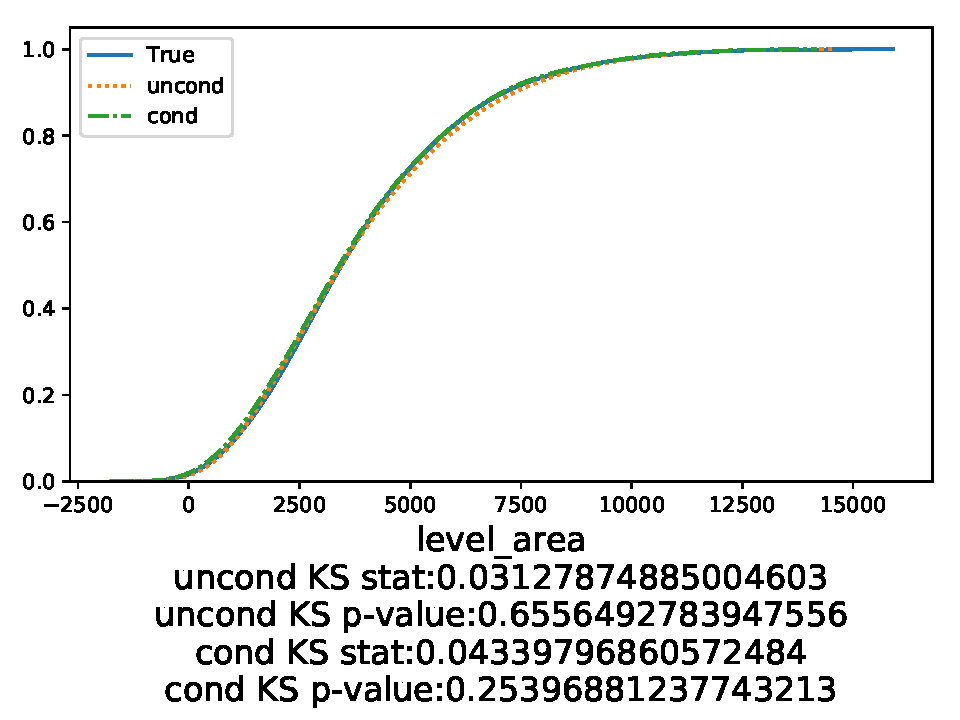
\includegraphics[width=\linewidth]{results/exp1-2/level_area.pdf} 
		\label{fig:results-noninput-level_area}
	\end{minipage}
	\begin{minipage}[b]{0.45\linewidth}
		\centering
		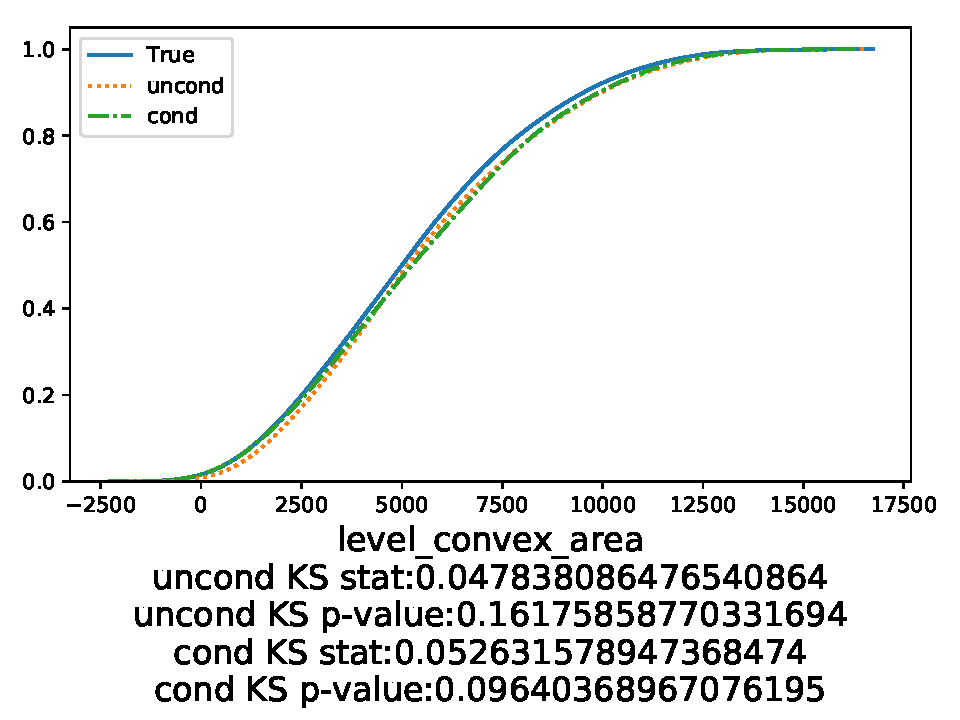
\includegraphics[width=\linewidth]{results/exp1-2/level_convex_area.pdf} 
		\label{fig:results-noninput-level_convex_area}
	\end{minipage} 
	
	
	\begin{minipage}[b]{0.45\linewidth}
		\centering
		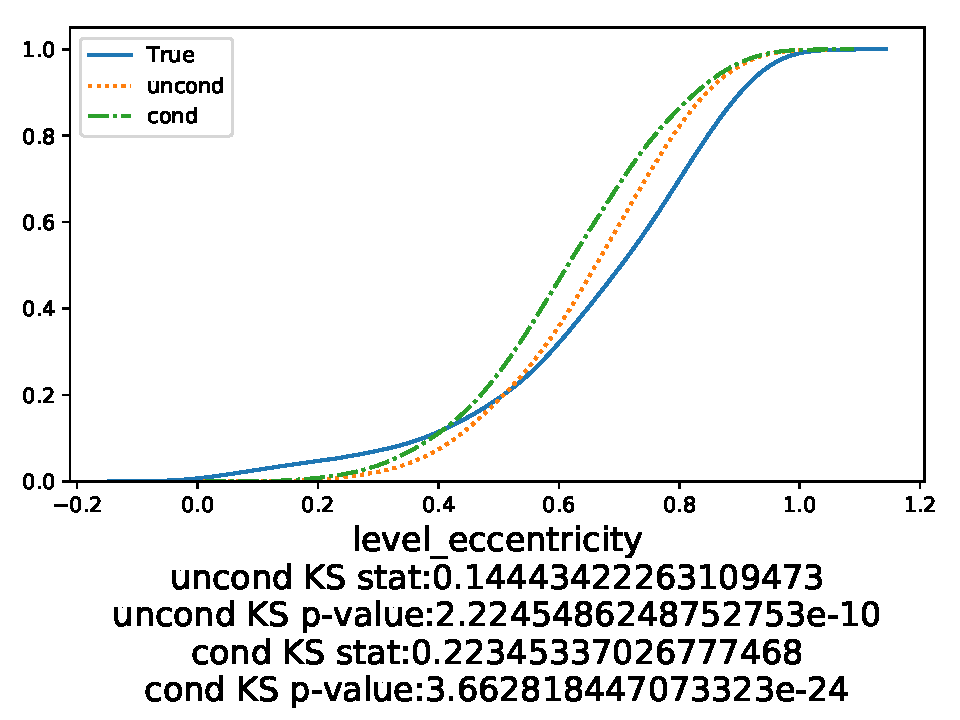
\includegraphics[width=\linewidth]{results/exp1-2/level_eccentricity.pdf} 
		\label{fig:results-noninput-level_eccentricity}
	\end{minipage}
	\begin{minipage}[b]{0.45\linewidth}
		\centering
		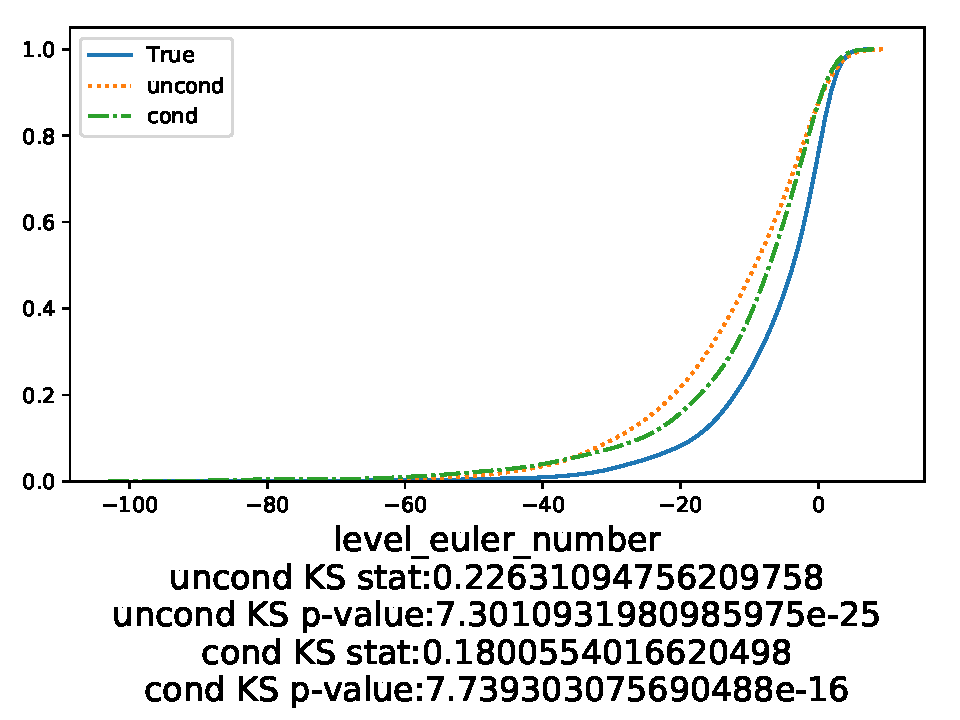
\includegraphics[width=\linewidth]{results/exp1-2/level_euler_number.pdf} 
		\label{fig:results-noninput-level_euler_number}
	\end{minipage} 
	
	
	\begin{minipage}[b]{0.45\linewidth}
		\centering
		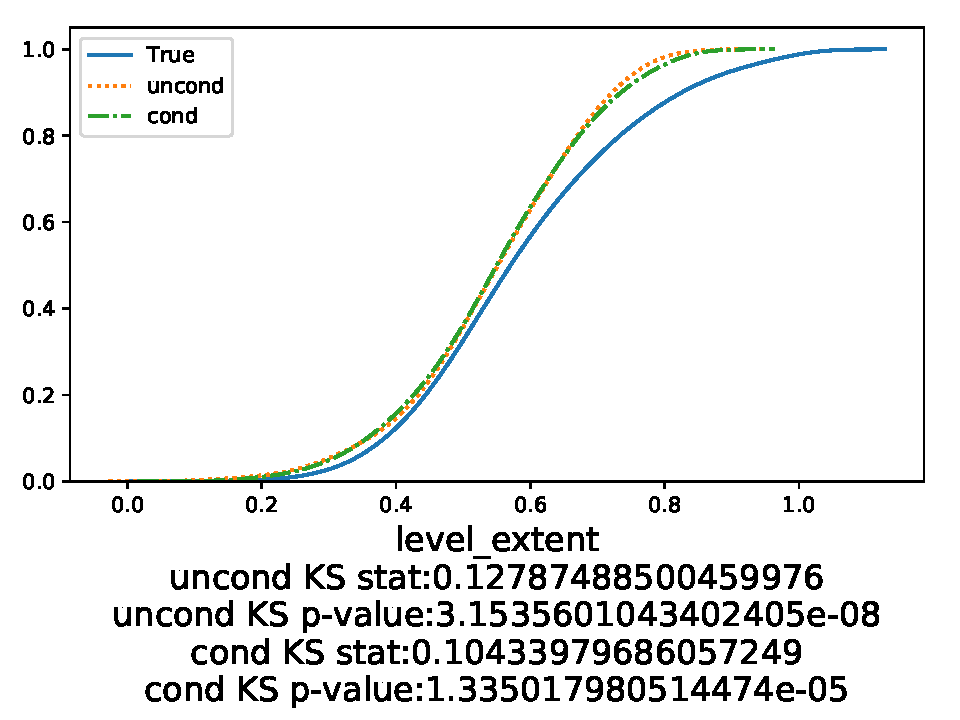
\includegraphics[width=\linewidth]{results/exp1-2/level_extent.pdf} 
		\label{fig:results-noninput-level_extent}
	\end{minipage}
	\begin{minipage}[b]{0.45\linewidth}
		\centering
		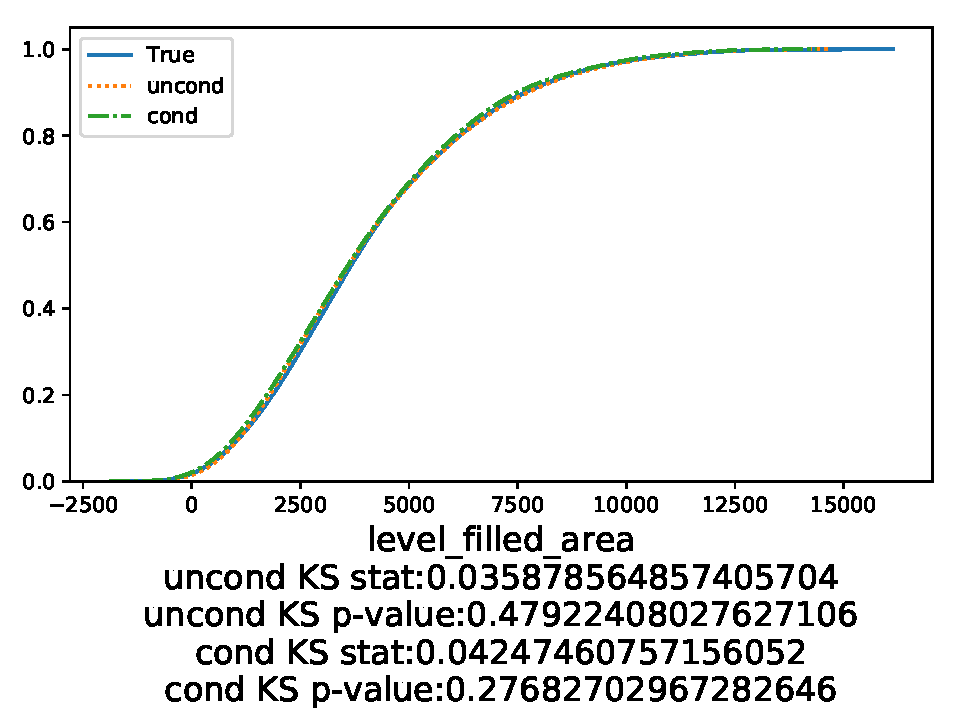
\includegraphics[width=\linewidth]{results/exp1-2/level_filled_area.pdf} 
		\label{fig:results-noninput-level_filled_area}
	\end{minipage} 
	
	
	\caption[Graphical results for experiments 1 and 2]{Experiments 1 and 2: Cumulative distribution functions for true data, unconditional network and conditional network for each non-input feature.}
\end{figure}\begin{figure}[ht]
	\begin{minipage}[b]{0.45\linewidth}
		\centering
		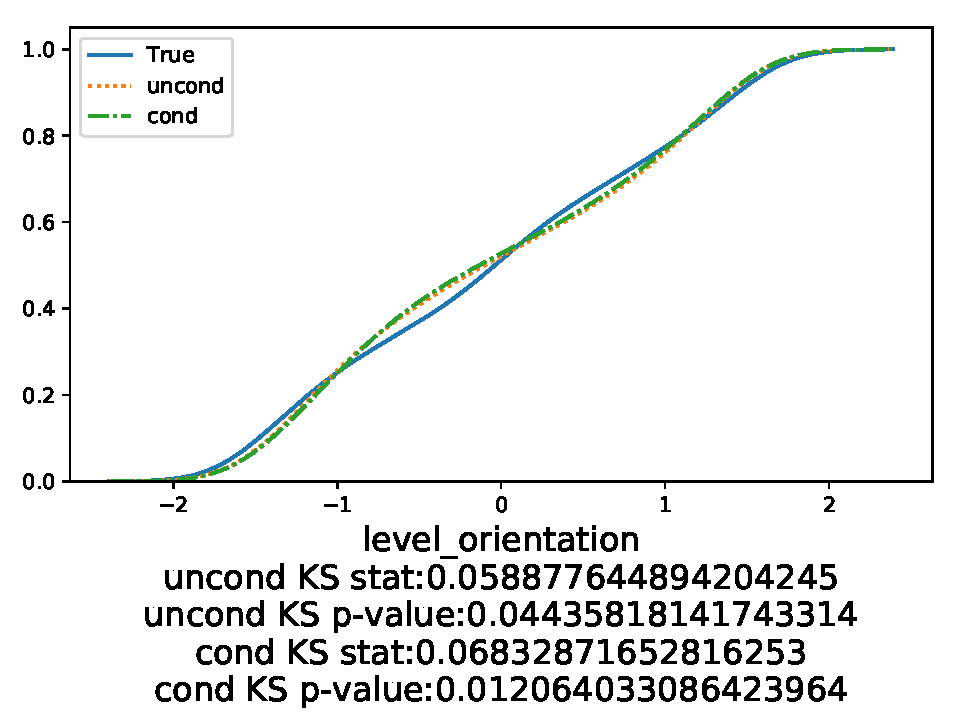
\includegraphics[width=\linewidth]{results/exp1-2/level_orientation.pdf} 
		\label{fig:results-noninput-level_orientation}
	\end{minipage}
	\begin{minipage}[b]{0.45\linewidth}
		\centering
		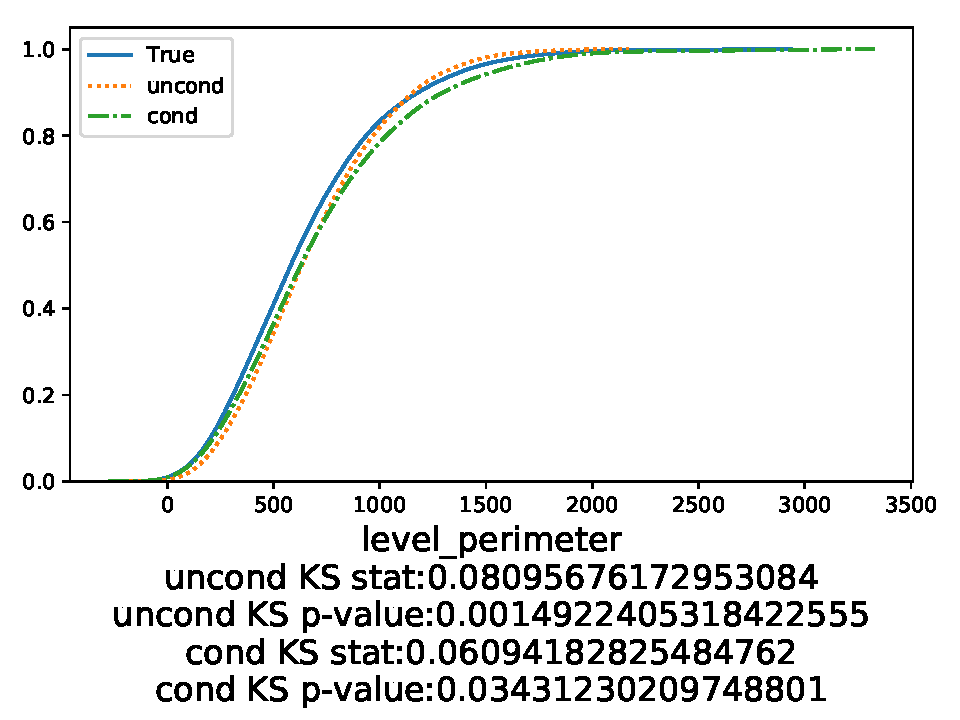
\includegraphics[width=\linewidth]{results/exp1-2/level_perimeter.pdf} 
		\label{fig:results-noninput-level_perimeter}
	\end{minipage} 
	
	
	\begin{minipage}[b]{0.45\linewidth}
		\centering
		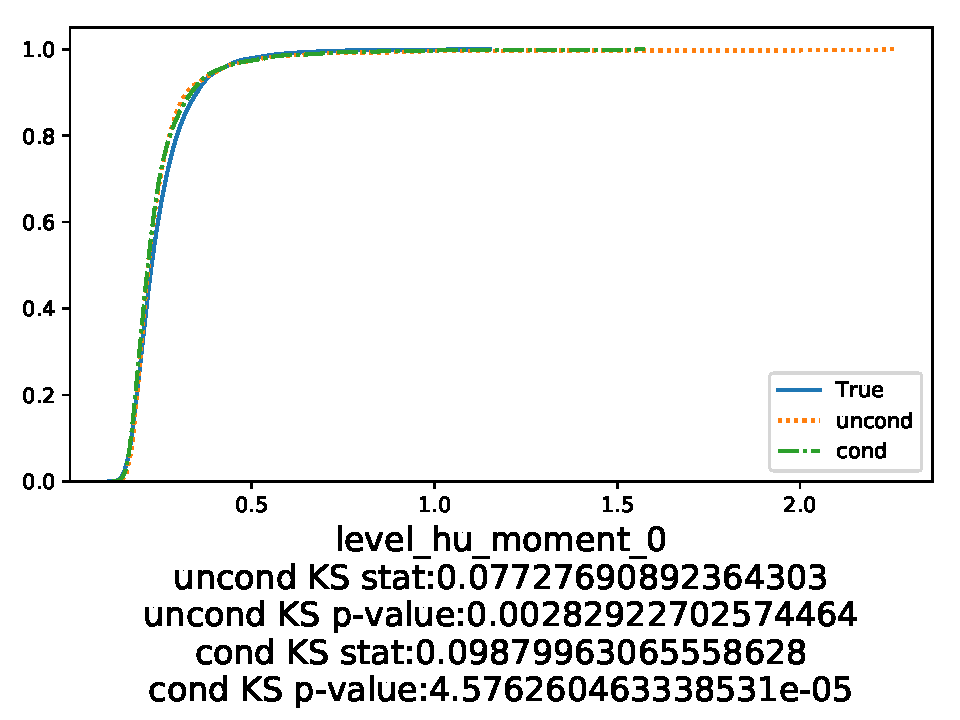
\includegraphics[width=\linewidth]{results/exp1-2/level_hu_moment_0.pdf} 
		\label{fig:results-noninput-level_hu_moment_0}
	\end{minipage}
	\begin{minipage}[b]{0.45\linewidth}
		\centering
		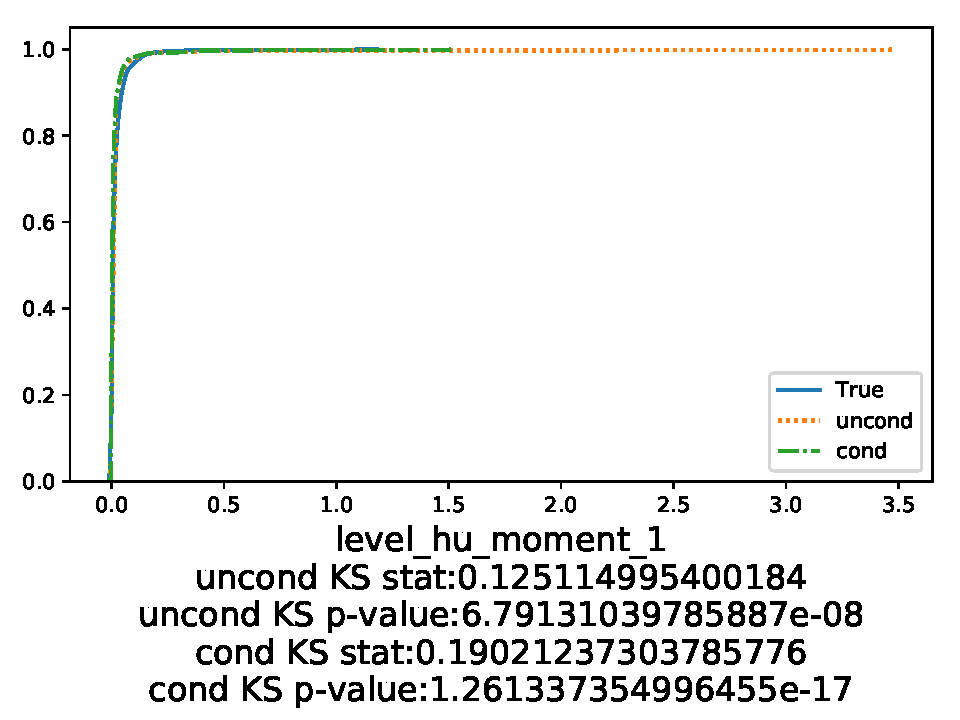
\includegraphics[width=\linewidth]{results/exp1-2/level_hu_moment_1.pdf} 
		\label{fig:results-noninput-level_hu_moment_1}
	\end{minipage} 
	
	
	\begin{minipage}[b]{0.45\linewidth}
		\centering
		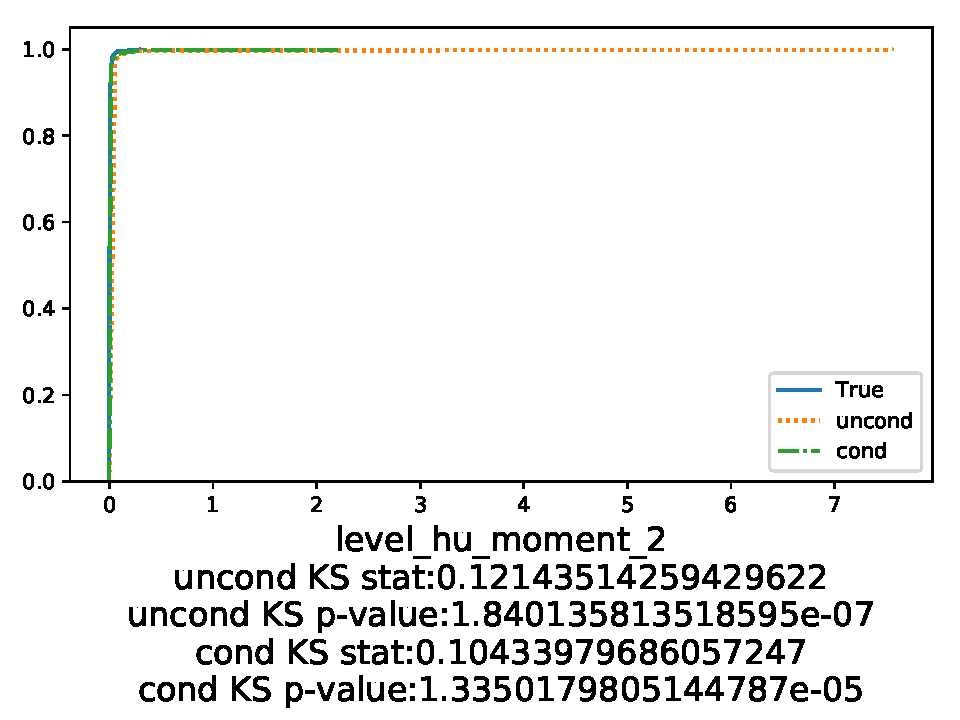
\includegraphics[width=\linewidth]{results/exp1-2/level_hu_moment_2.pdf} 
		\label{fig:results-noninput-level_hu_moment_2}
	\end{minipage}
	\begin{minipage}[b]{0.45\linewidth}
		\centering
		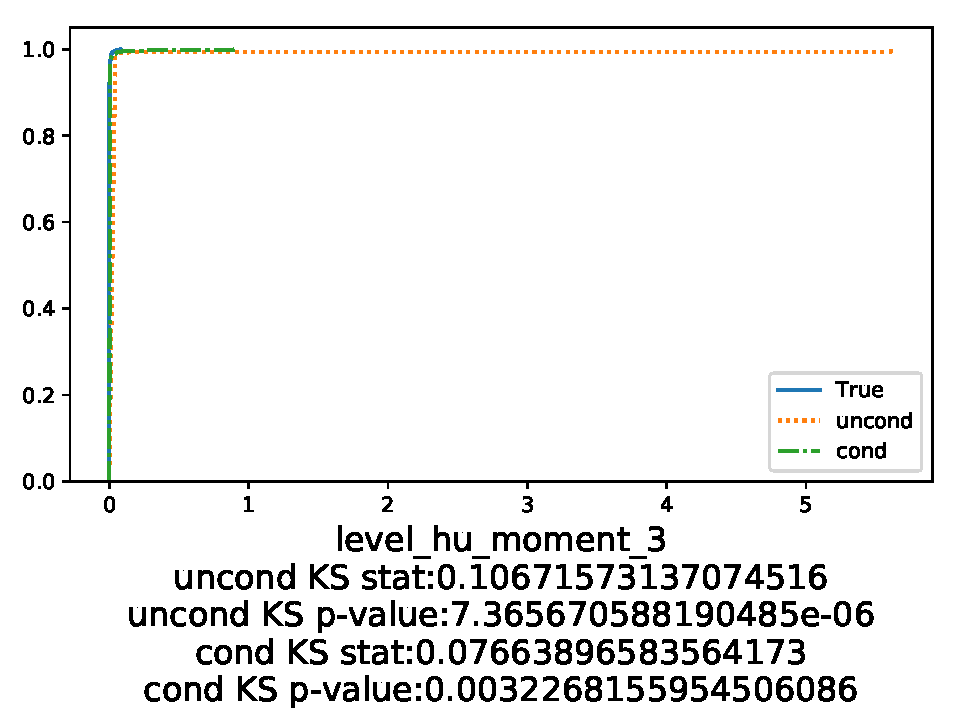
\includegraphics[width=\linewidth]{results/exp1-2/level_hu_moment_3.pdf} 
		\label{fig:results-noninput-level_hu_moment_3}
	\end{minipage} 
	
	
	\caption[Graphical results for experiments 1 and 2]{Experiments 1 and 2: Cumulative distribution functions for true data, unconditional network and conditional network for each non-input feature.}
\end{figure}\begin{figure}[ht]
	\begin{minipage}[b]{0.45\linewidth}
		\centering
		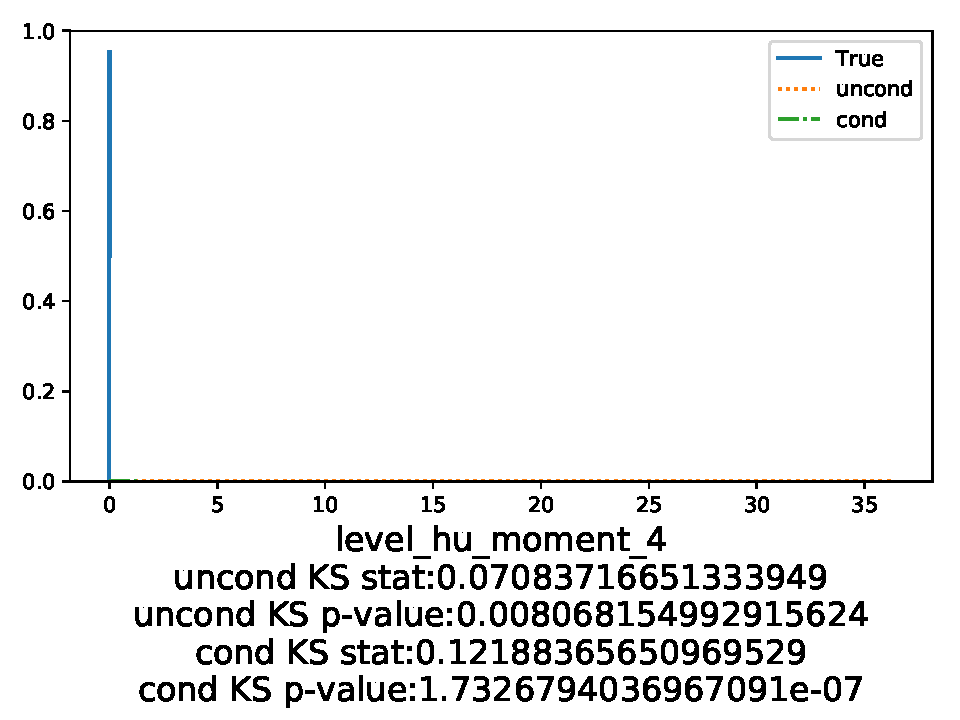
\includegraphics[width=\linewidth]{results/exp1-2/level_hu_moment_4.pdf} 
		\label{fig:results-noninput-level_hu_moment_4}
	\end{minipage}
	\begin{minipage}[b]{0.45\linewidth}
		\centering
		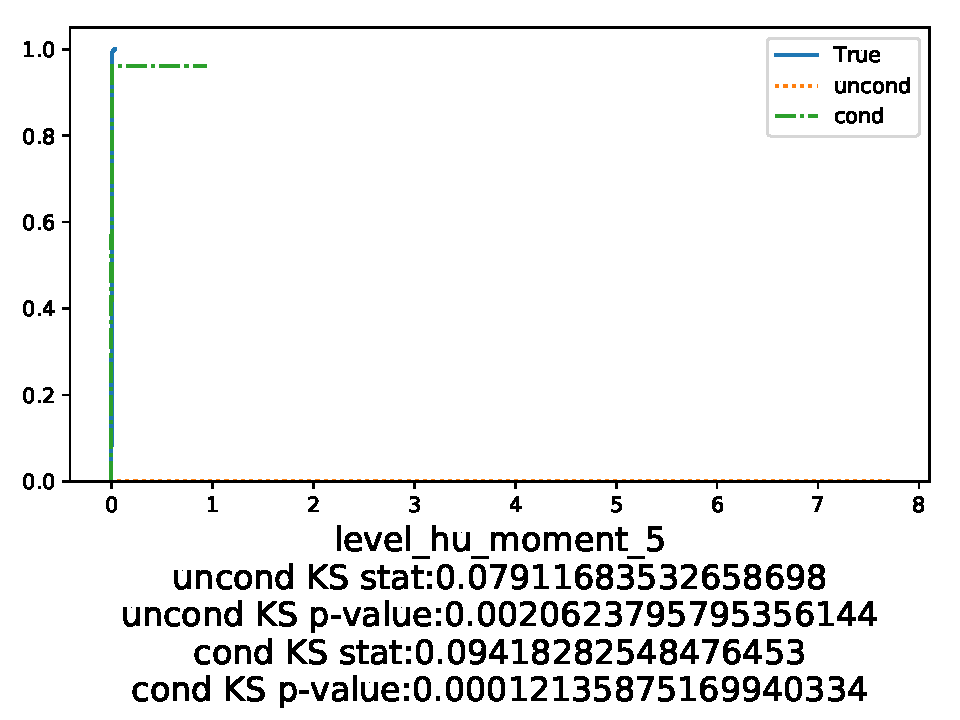
\includegraphics[width=\linewidth]{results/exp1-2/level_hu_moment_5.pdf} 
		\label{fig:results-noninput-level_hu_moment_5}
	\end{minipage} 
	
	
	\begin{minipage}[b]{0.45\linewidth}
		\centering
		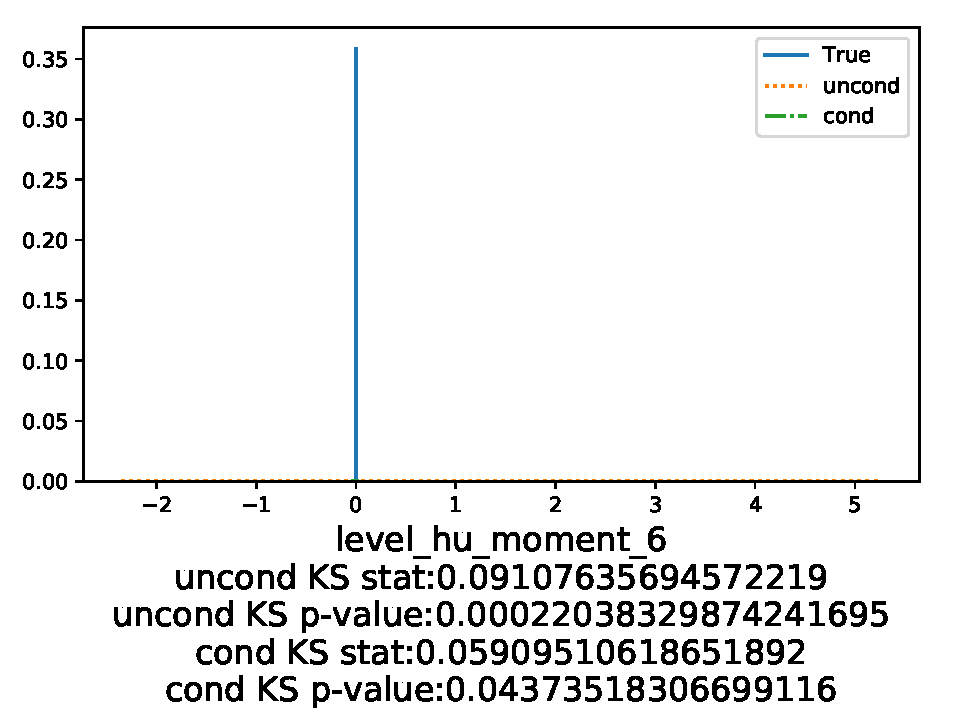
\includegraphics[width=\linewidth]{results/exp1-2/level_hu_moment_6.pdf} 
		\label{fig:results-noninput-level_hu_moment_6}
	\end{minipage}
	\begin{minipage}[b]{0.45\linewidth}
		\centering
		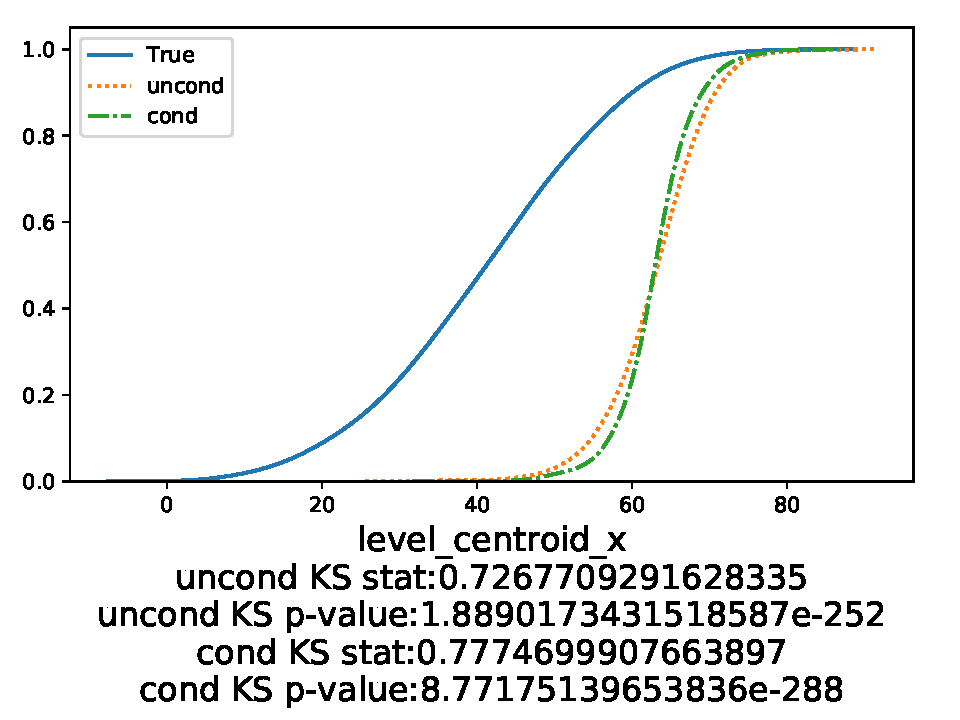
\includegraphics[width=\linewidth]{results/exp1-2/level_centroid_x.pdf} 
		\label{fig:results-noninput-level_centroid_x}
	\end{minipage} 
	
	
	\begin{minipage}[b]{0.45\linewidth}
		\centering
		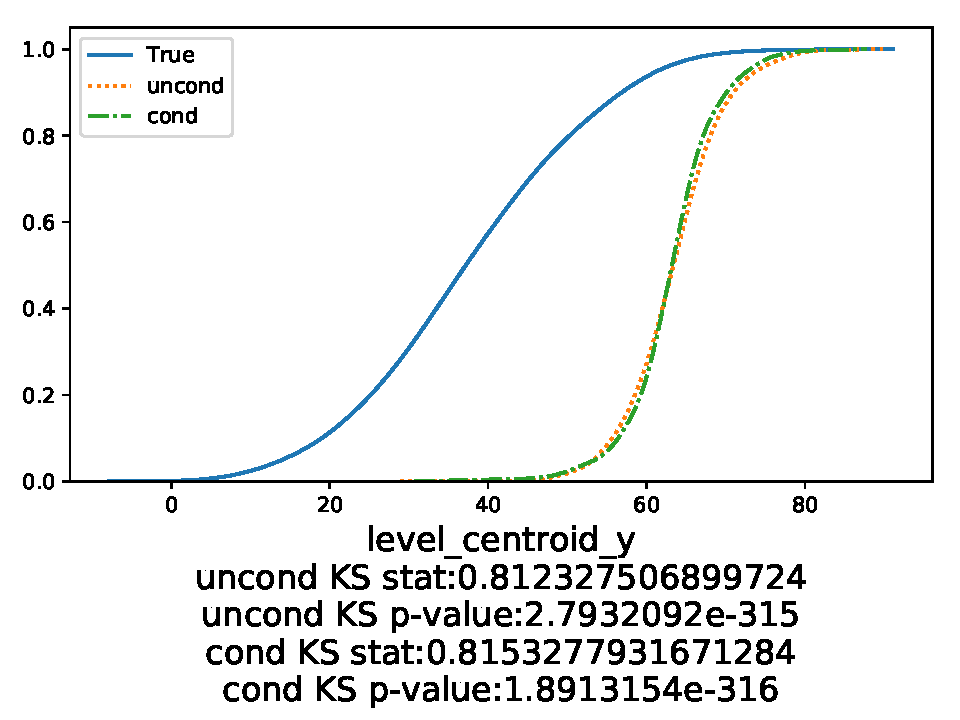
\includegraphics[width=\linewidth]{results/exp1-2/level_centroid_y.pdf} 
		\label{fig:results-noninput-level_centroid_y}
	\end{minipage}
	\begin{minipage}[b]{0.45\linewidth}
		\centering
		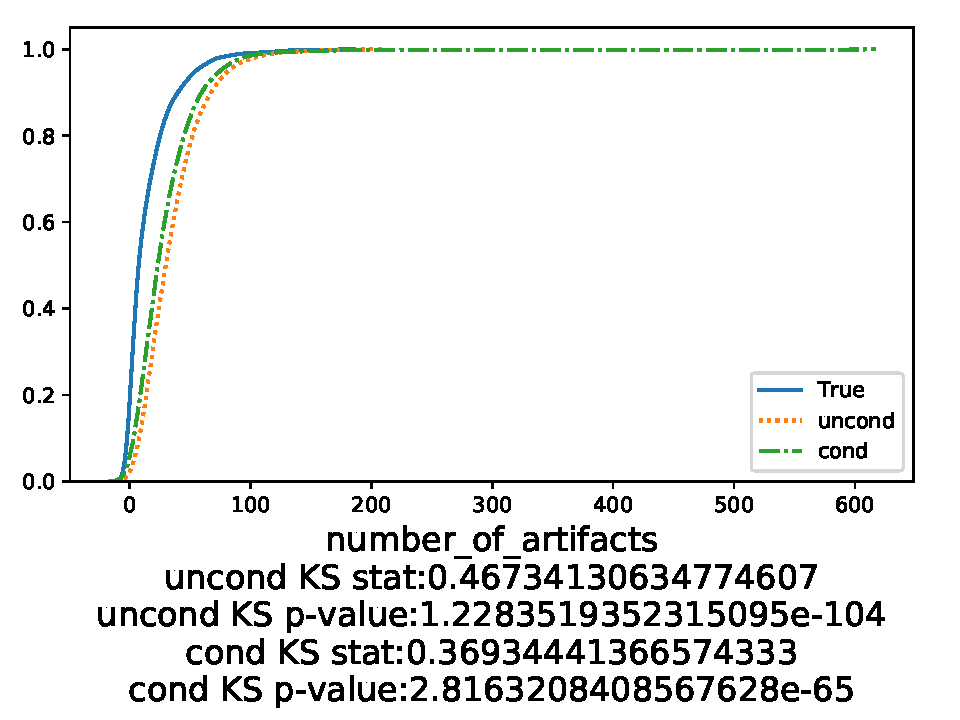
\includegraphics[width=\linewidth]{results/exp1-2/number_of_artifacts.pdf} 
		\label{fig:results-noninput-number_of_artifacts}
	\end{minipage} 
	
	
	\caption[Graphical results for experiments 1 and 2]{Experiments 1 and 2: Cumulative distribution functions for true data, unconditional network and conditional network for each non-input feature.}
\end{figure}\begin{figure}[ht]
	\begin{minipage}[b]{0.45\linewidth}
		\centering
		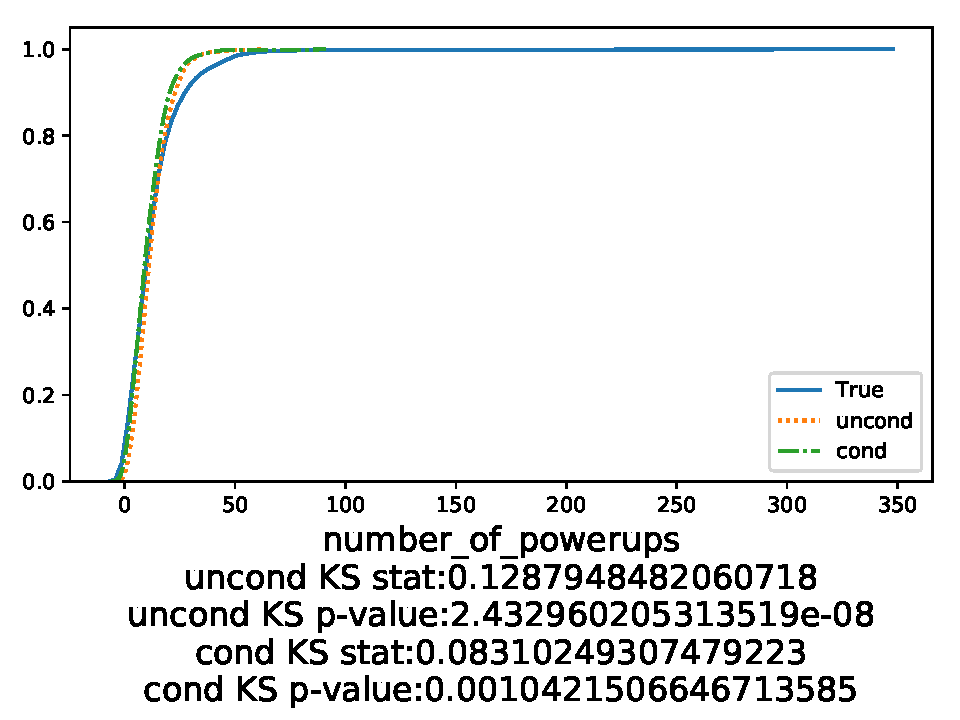
\includegraphics[width=\linewidth]{results/exp1-2/number_of_powerups.pdf} 
		\label{fig:results-noninput-number_of_powerups}
	\end{minipage}
	\begin{minipage}[b]{0.45\linewidth}
		\centering
		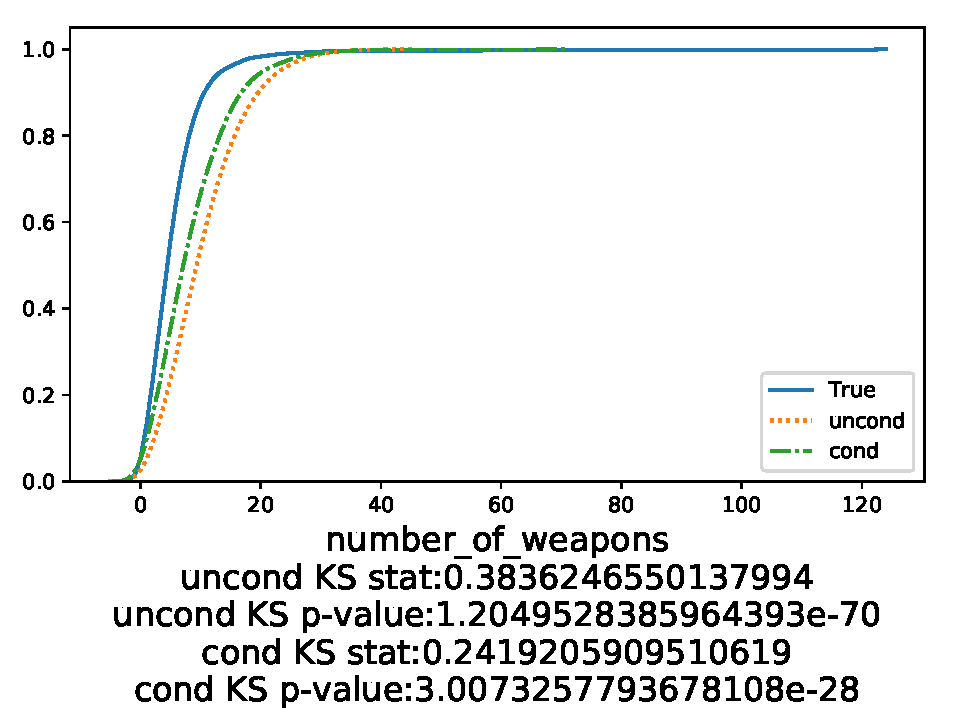
\includegraphics[width=\linewidth]{results/exp1-2/number_of_weapons.pdf} 
		\label{fig:results-noninput-number_of_weapons}
	\end{minipage} 
	
	
	\begin{minipage}[b]{0.45\linewidth}
		\centering
		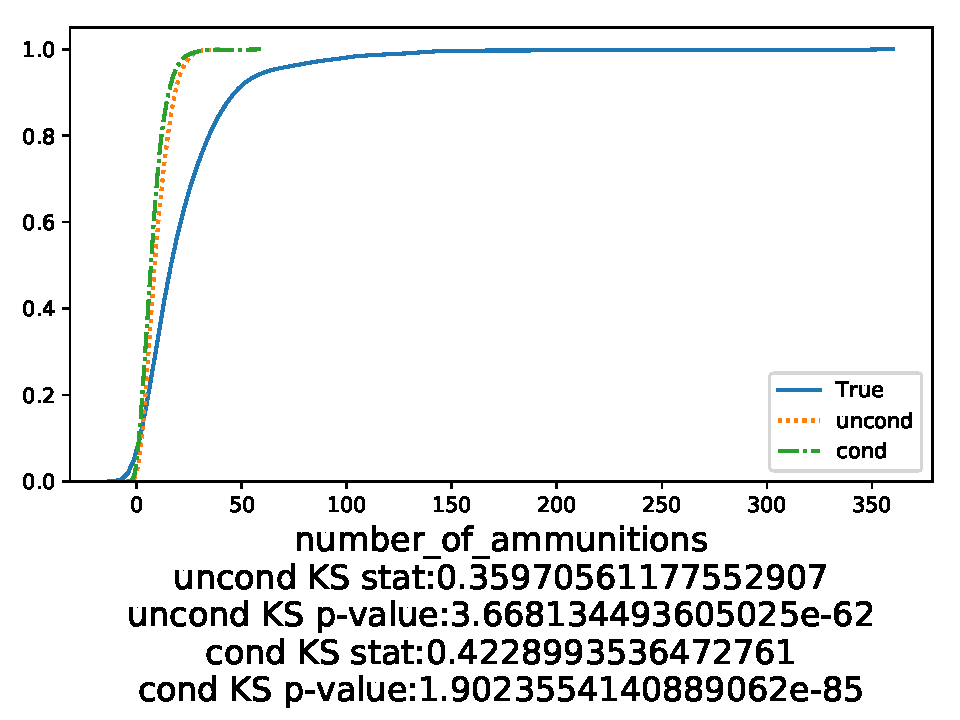
\includegraphics[width=\linewidth]{results/exp1-2/number_of_ammunitions.pdf} 
		\label{fig:results-noninput-number_of_ammunitions}
	\end{minipage}
	\begin{minipage}[b]{0.45\linewidth}
		\centering
		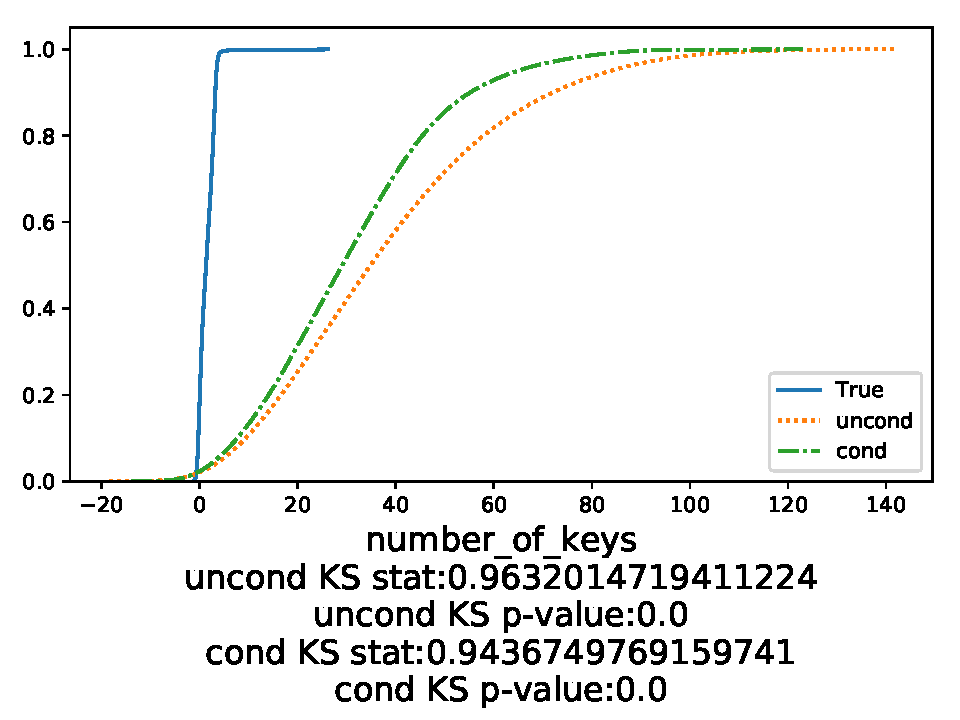
\includegraphics[width=\linewidth]{results/exp1-2/number_of_keys.pdf} 
		\label{fig:results-noninput-number_of_keys}
	\end{minipage} 
	
	
	\begin{minipage}[b]{0.45\linewidth}
		\centering
		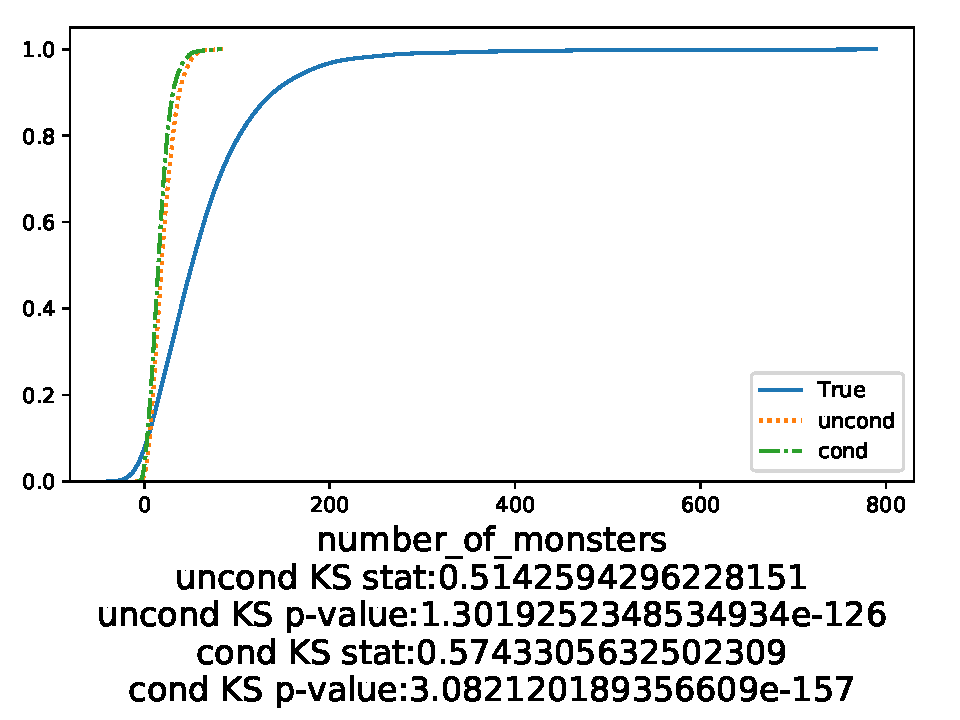
\includegraphics[width=\linewidth]{results/exp1-2/number_of_monsters.pdf} 
		\label{fig:results-noninput-number_of_monsters}
	\end{minipage}
	\begin{minipage}[b]{0.45\linewidth}
		\centering
		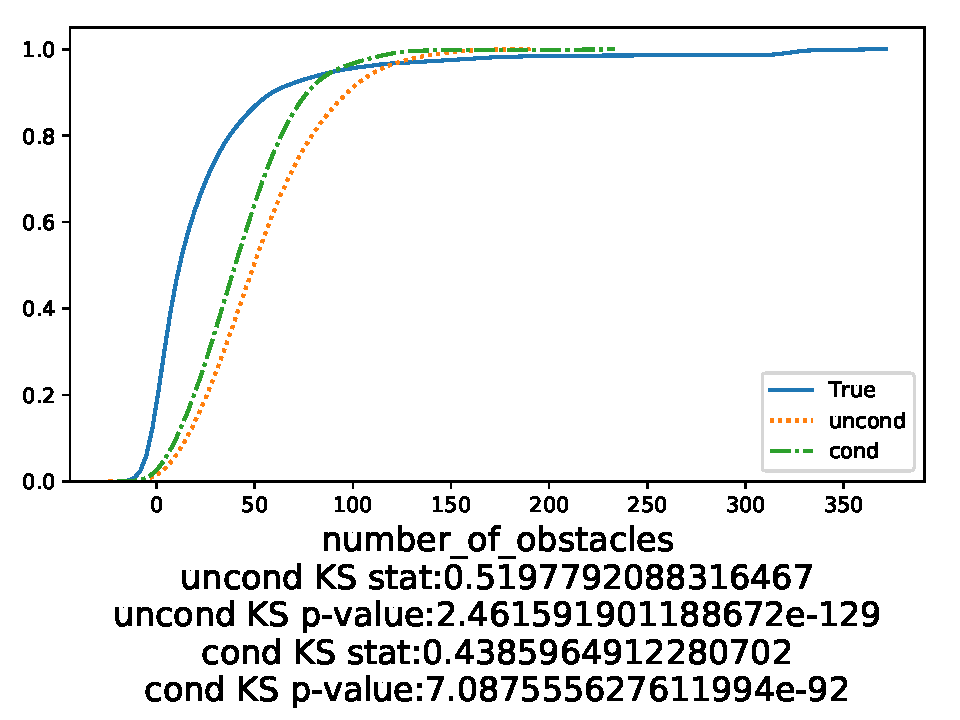
\includegraphics[width=\linewidth]{results/exp1-2/number_of_obstacles.pdf} 
		\label{fig:results-noninput-number_of_obstacles}
	\end{minipage} 
	
	
	\caption[Graphical results for experiments 1 and 2]{Experiments 1 and 2: Cumulative distribution functions for true data, unconditional network and conditional network for each non-input feature.}
\end{figure}\begin{figure}[ht]
	\begin{minipage}[b]{0.45\linewidth}
		\centering
		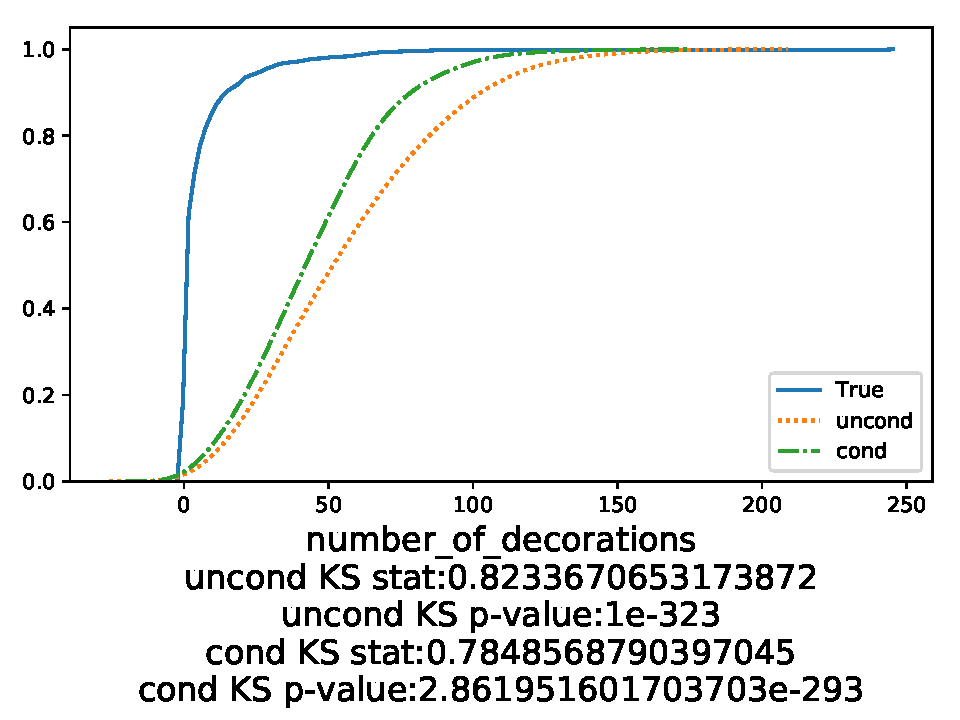
\includegraphics[width=\linewidth]{results/exp1-2/number_of_decorations.pdf} 
		\label{fig:results-noninput-number_of_decorations}
	\end{minipage}
	\begin{minipage}[b]{0.45\linewidth}
		\centering
		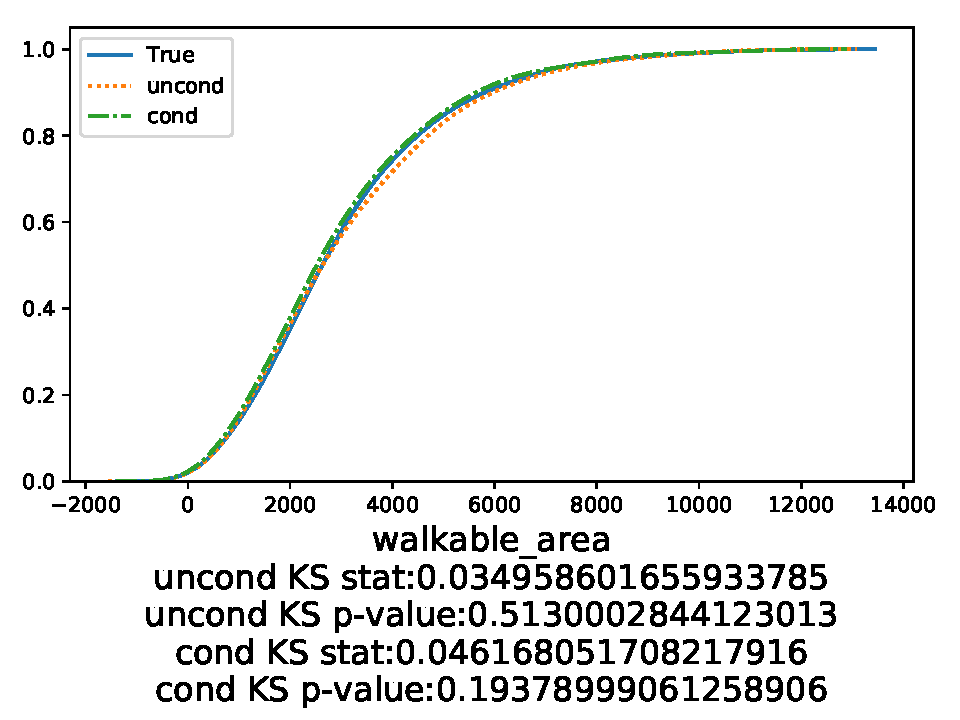
\includegraphics[width=\linewidth]{results/exp1-2/walkable_area.pdf} 
		\label{fig:results-noninput-walkable_area}
	\end{minipage} 
	
	
	\begin{minipage}[b]{0.45\linewidth}
		\centering
		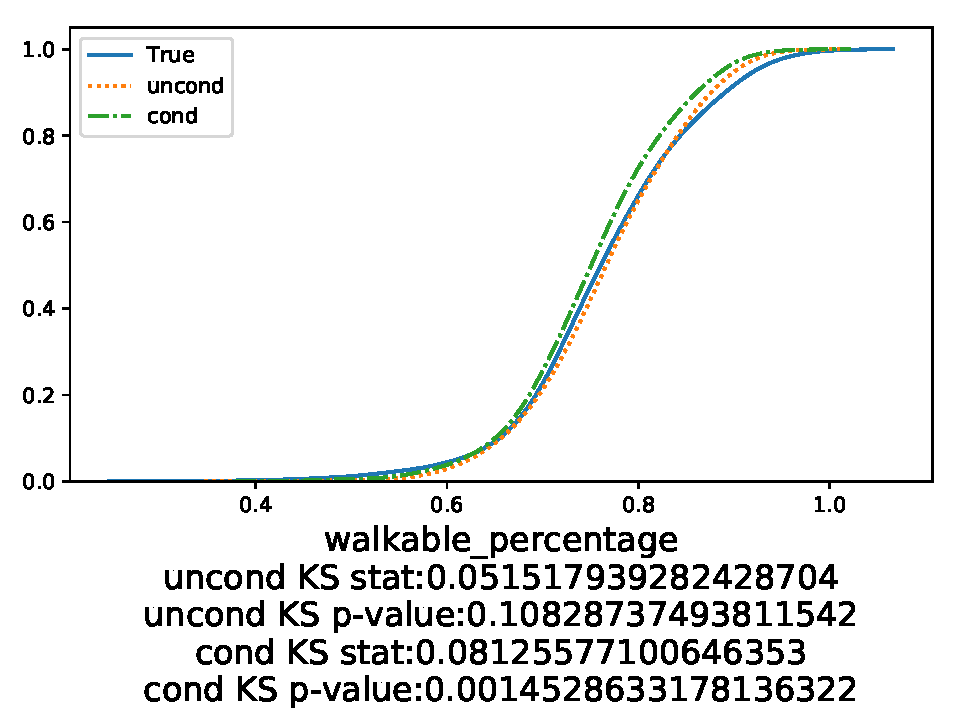
\includegraphics[width=\linewidth]{results/exp1-2/walkable_percentage.pdf} 
		\label{fig:results-noninput-walkable_percentage}
	\end{minipage}
	\begin{minipage}[b]{0.45\linewidth}
		\centering
		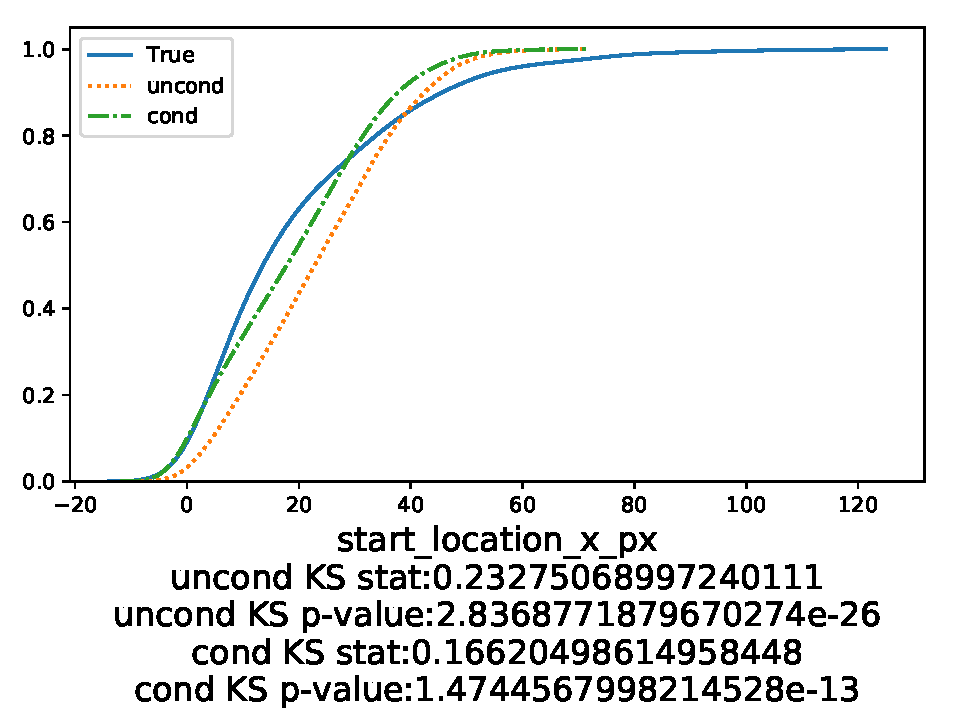
\includegraphics[width=\linewidth]{results/exp1-2/start_location_x_px.pdf} 
		\label{fig:results-noninput-start_location_x_px}
	\end{minipage} 
	
	
	\begin{minipage}[b]{0.45\linewidth}
		\centering
		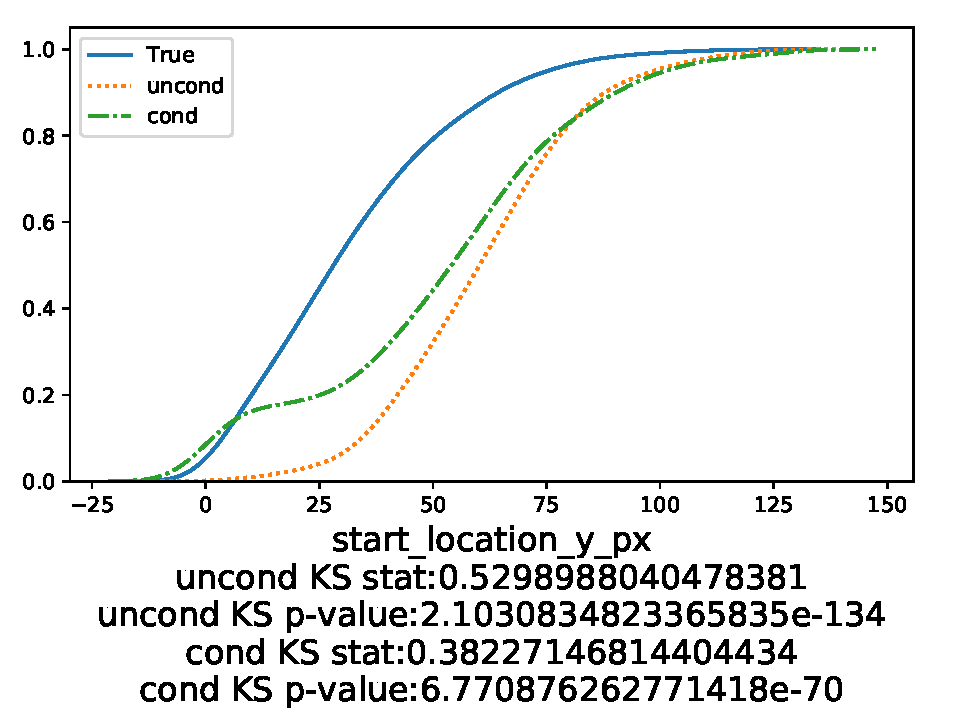
\includegraphics[width=\linewidth]{results/exp1-2/start_location_y_px.pdf} 
		\label{fig:results-noninput-start_location_y_px}
	\end{minipage}
	\begin{minipage}[b]{0.45\linewidth}
		\centering
		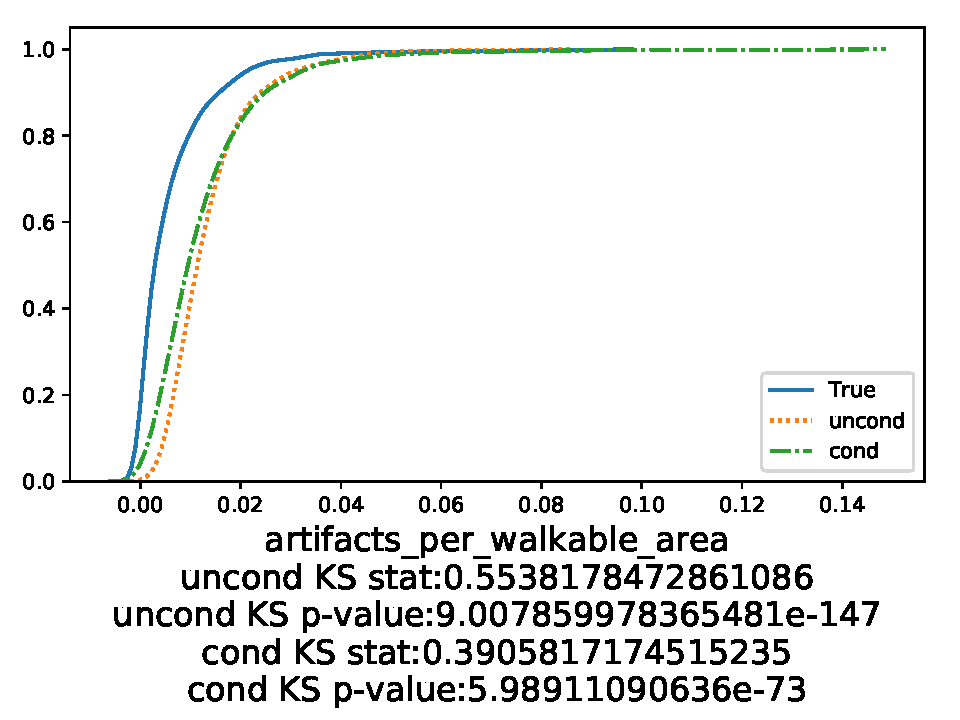
\includegraphics[width=\linewidth]{results/exp1-2/artifacts_per_walkable_area.pdf} 
		\label{fig:results-noninput-artifacts_per_walkable_area}
	\end{minipage} 
	
	
	\caption[Graphical results for experiments 1 and 2]{Experiments 1 and 2: Cumulative distribution functions for true data, unconditional network and conditional network for each non-input feature.}
\end{figure}\begin{figure}[ht]
	\begin{minipage}[b]{0.45\linewidth}
		\centering
		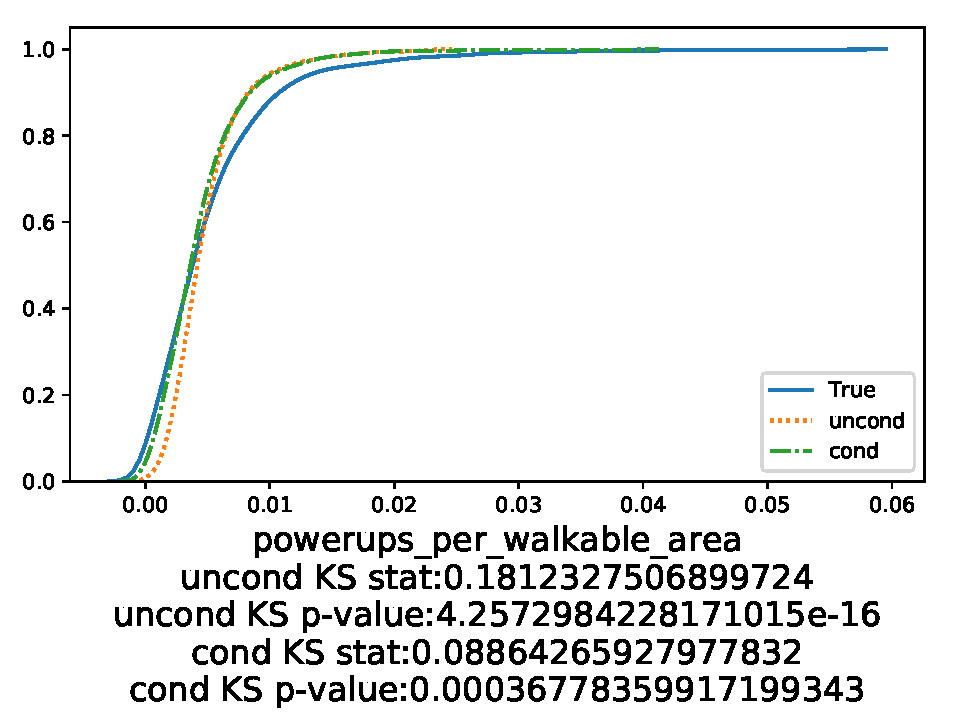
\includegraphics[width=\linewidth]{results/exp1-2/powerups_per_walkable_area.pdf} 
		\label{fig:results-noninput-powerups_per_walkable_area}
	\end{minipage}
	\begin{minipage}[b]{0.45\linewidth}
		\centering
		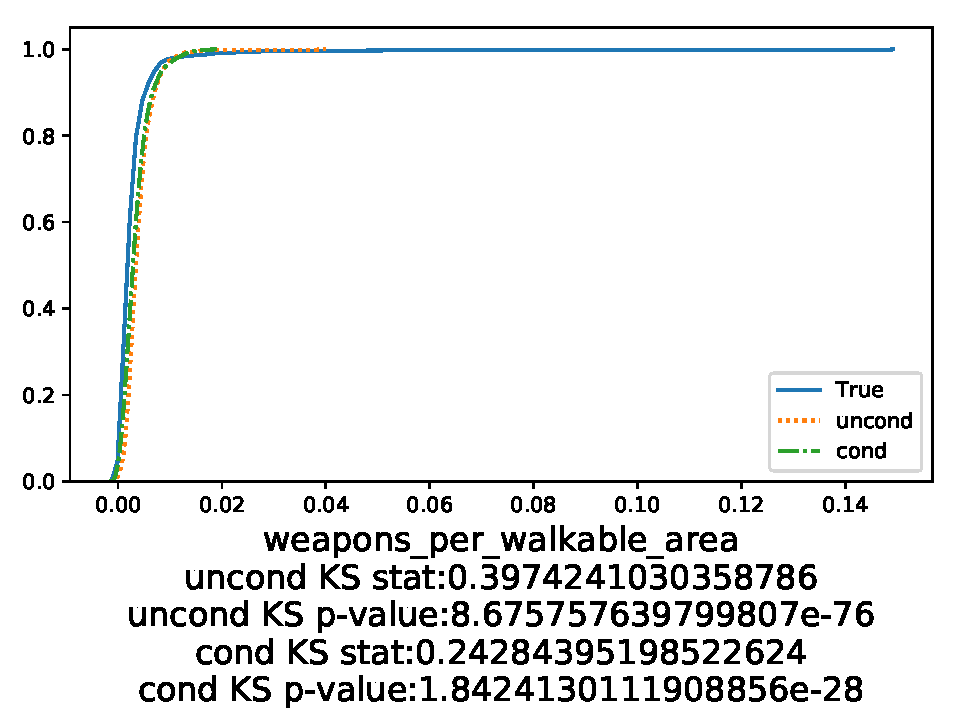
\includegraphics[width=\linewidth]{results/exp1-2/weapons_per_walkable_area.pdf} 
		\label{fig:results-noninput-weapons_per_walkable_area}
	\end{minipage} 
	
	
	\begin{minipage}[b]{0.45\linewidth}
		\centering
		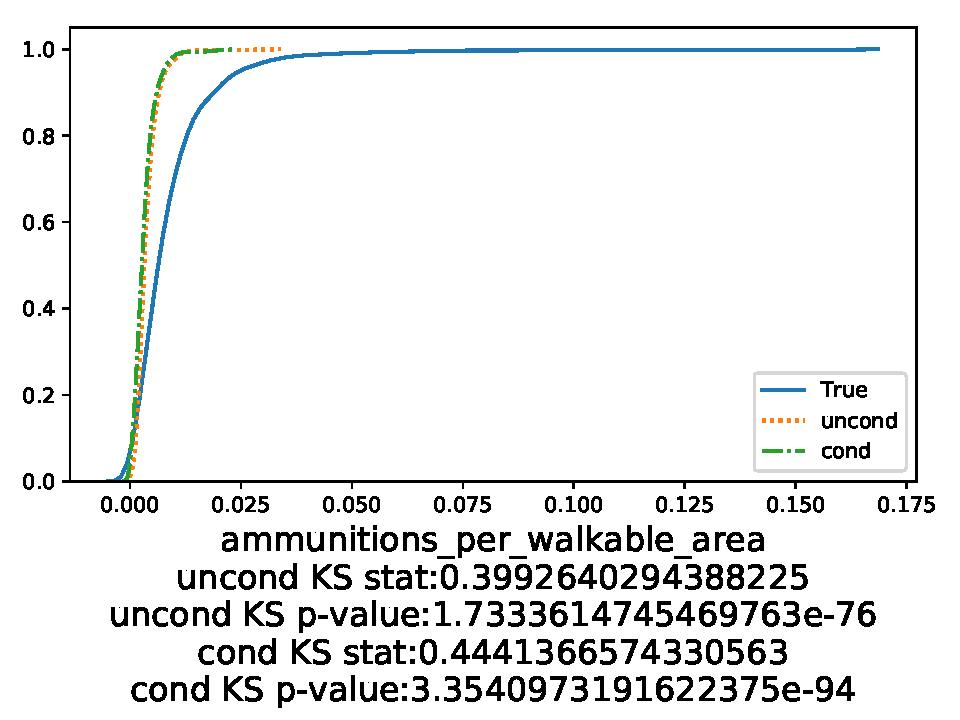
\includegraphics[width=\linewidth]{results/exp1-2/ammunitions_per_walkable_area.pdf} 
		\label{fig:results-noninput-ammunitions_per_walkable_area}
	\end{minipage}
	\begin{minipage}[b]{0.45\linewidth}
		\centering
		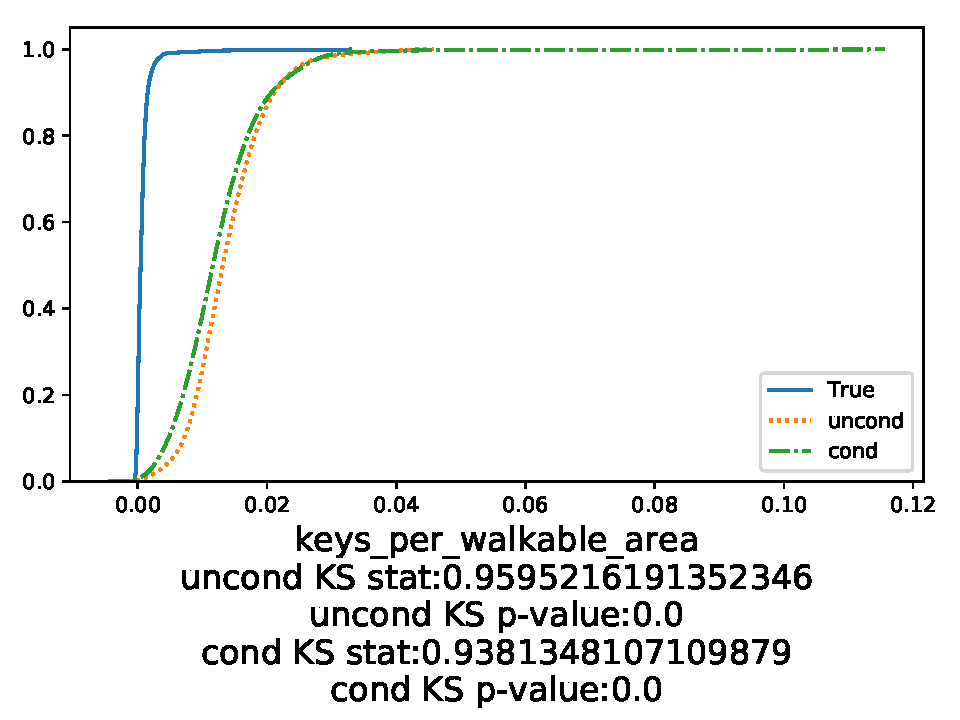
\includegraphics[width=\linewidth]{results/exp1-2/keys_per_walkable_area.pdf} 
		\label{fig:results-noninput-keys_per_walkable_area}
	\end{minipage} 
	
	
	\begin{minipage}[b]{0.45\linewidth}
		\centering
		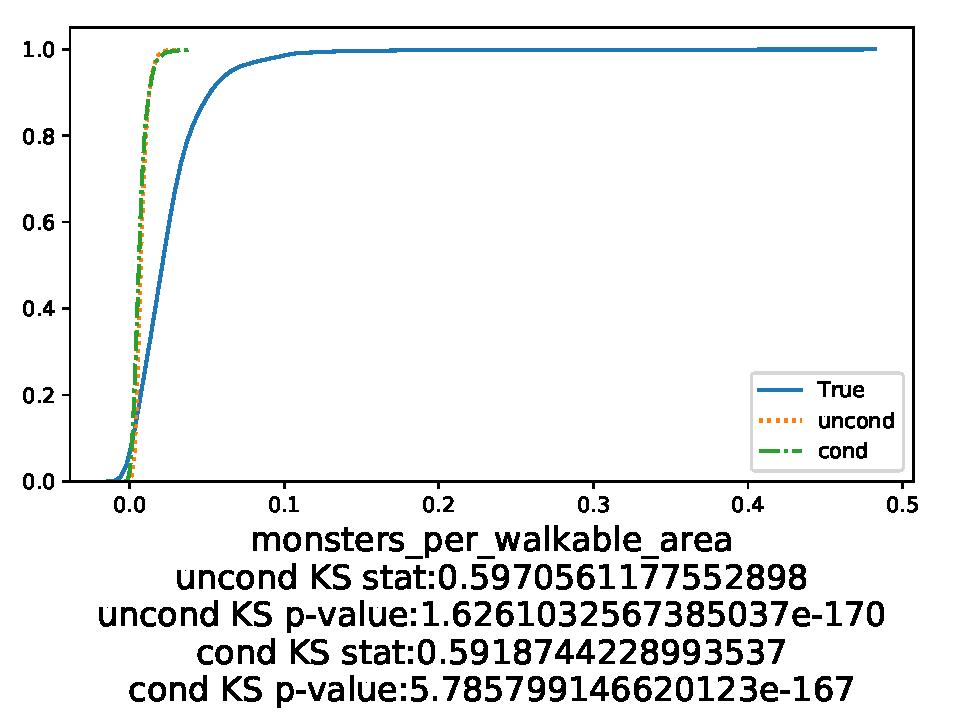
\includegraphics[width=\linewidth]{results/exp1-2/monsters_per_walkable_area.pdf} 
		\label{fig:results-noninput-monsters_per_walkable_area}
	\end{minipage}
	\begin{minipage}[b]{0.45\linewidth}
		\centering
		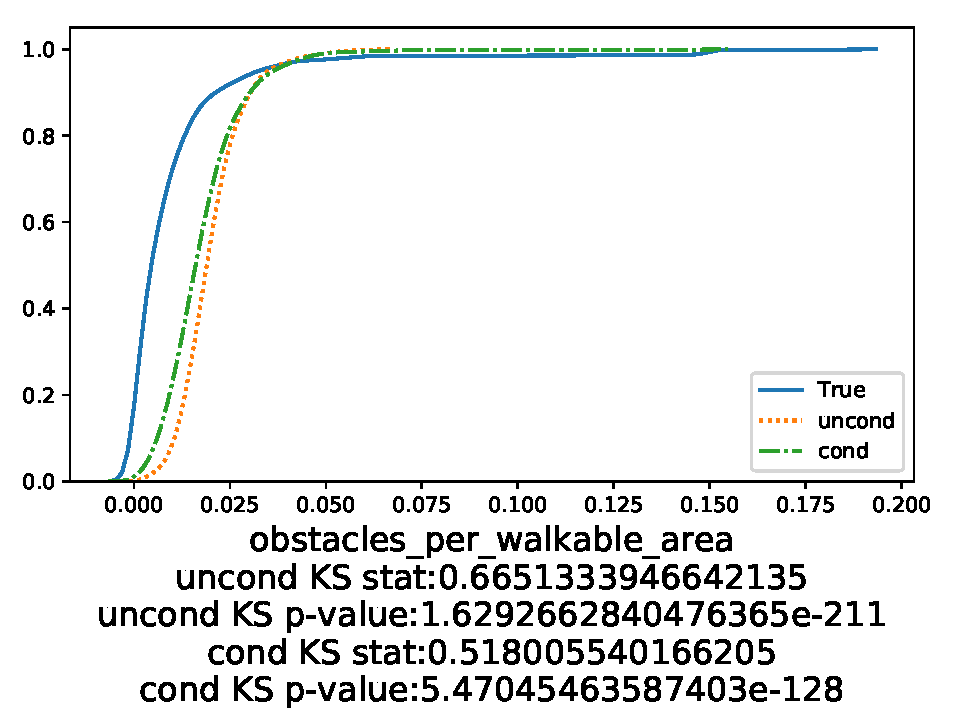
\includegraphics[width=\linewidth]{results/exp1-2/obstacles_per_walkable_area.pdf} 
		\label{fig:results-noninput-obstacles_per_walkable_area}
	\end{minipage} 
	
	
	\caption[Graphical results for experiments 1 and 2]{Experiments 1 and 2: Cumulative distribution functions for true data, unconditional network and conditional network for each non-input feature.}
\end{figure}\begin{figure}[ht]
	\begin{minipage}[b]{0.45\linewidth}
		\centering
		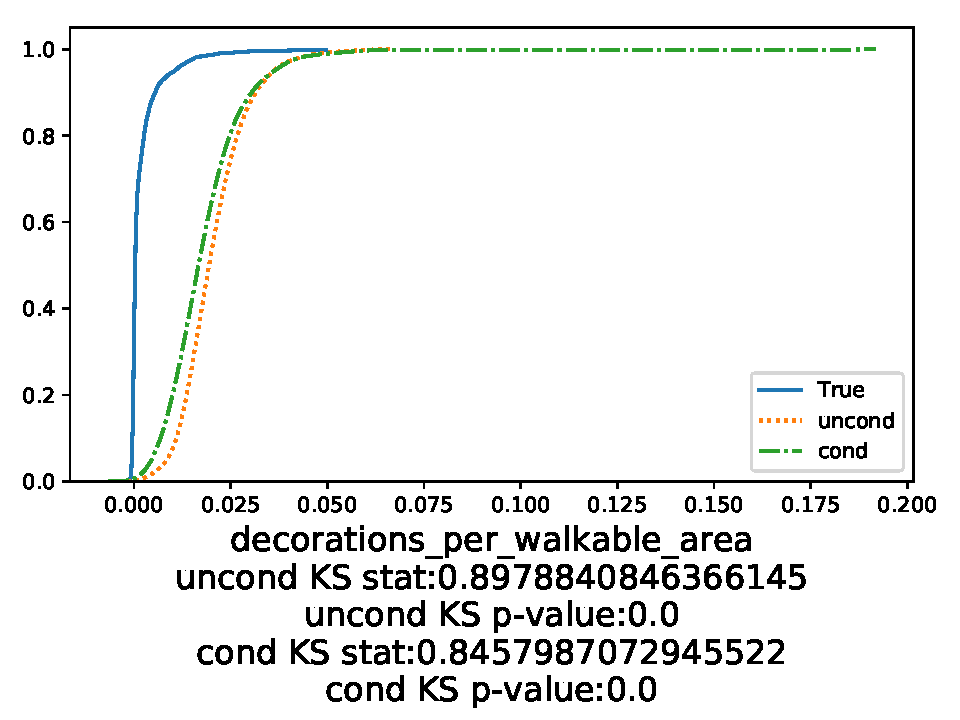
\includegraphics[width=\linewidth]{results/exp1-2/decorations_per_walkable_area.pdf} 
		\label{fig:results-noninput-decorations_per_walkable_area}
	\end{minipage}
	\begin{minipage}[b]{0.45\linewidth}
		\centering
		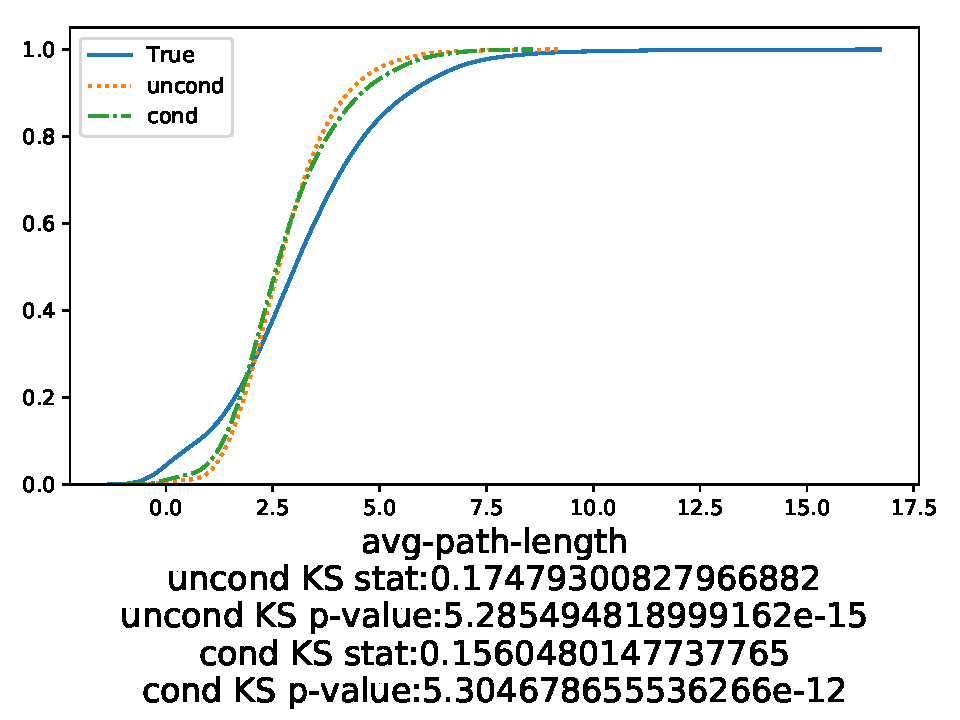
\includegraphics[width=\linewidth]{results/exp1-2/avg-path-length.pdf} 
		\label{fig:results-noninput-avg-path-length}
	\end{minipage} 
	
	
	\begin{minipage}[b]{0.45\linewidth}
		\centering
		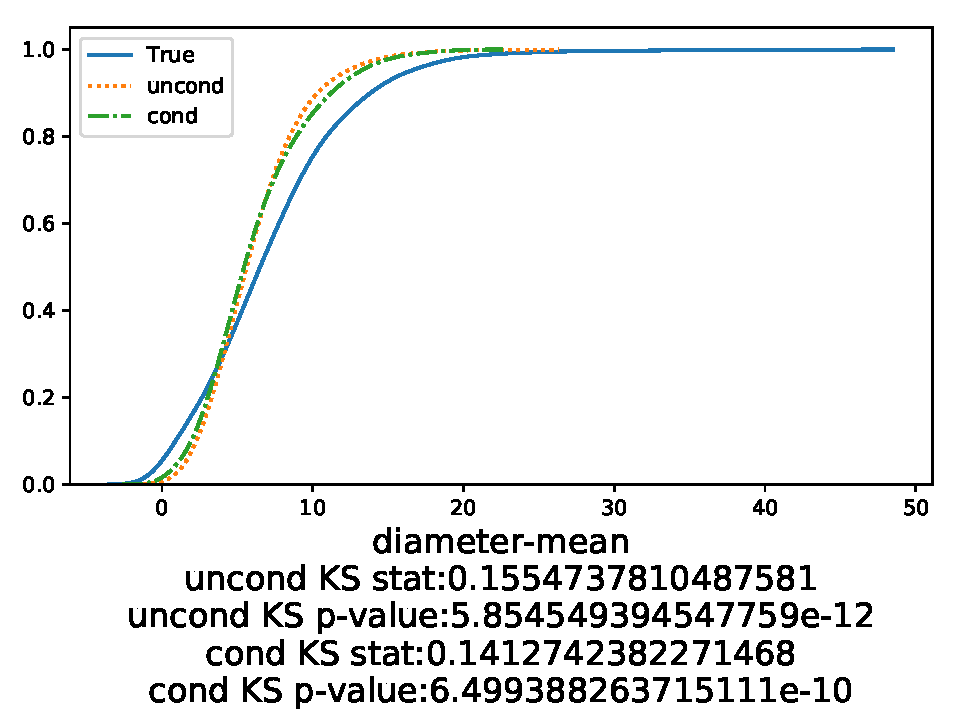
\includegraphics[width=\linewidth]{results/exp1-2/diameter-mean.pdf} 
		\label{fig:results-noninput-diameter-mean}
	\end{minipage}
	\begin{minipage}[b]{0.45\linewidth}
		\centering
		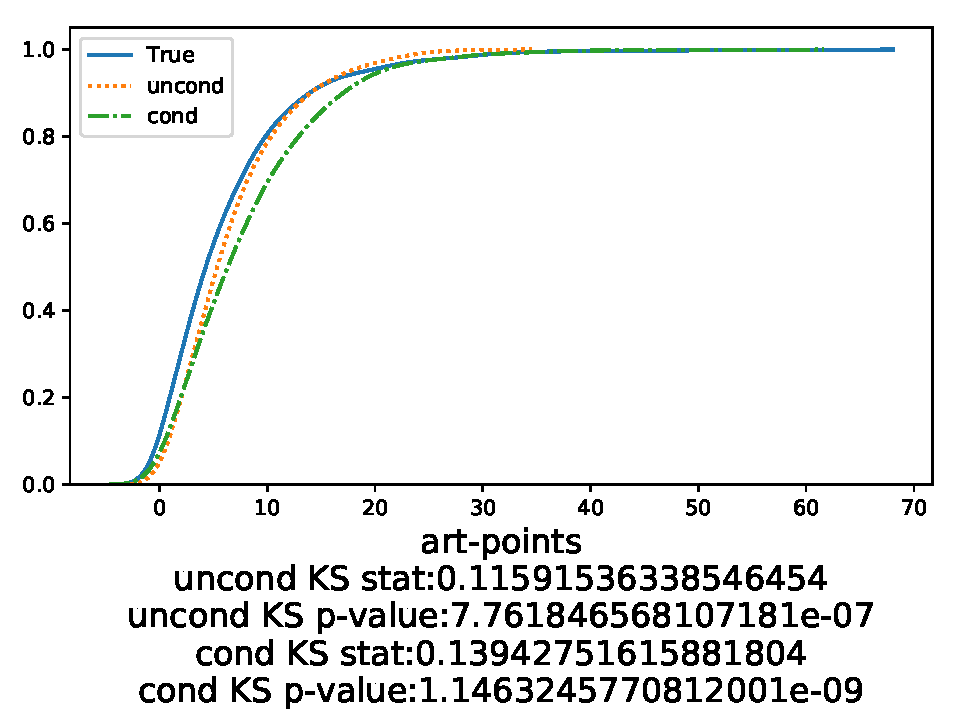
\includegraphics[width=\linewidth]{results/exp1-2/art-points.pdf} 
		\label{fig:results-noninput-art-points}
	\end{minipage} 
	
	
	\begin{minipage}[b]{0.45\linewidth}
		\centering
		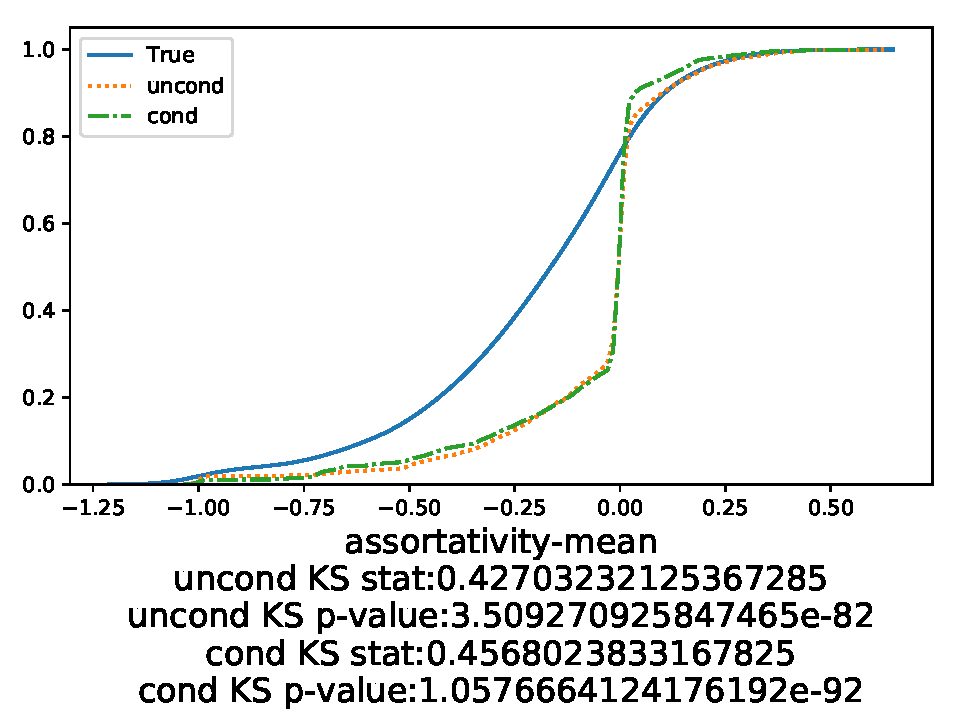
\includegraphics[width=\linewidth]{results/exp1-2/assortativity-mean.pdf} 
		\label{fig:results-noninput-assortativity-mean}
	\end{minipage}
	\begin{minipage}[b]{0.45\linewidth}
		\centering
		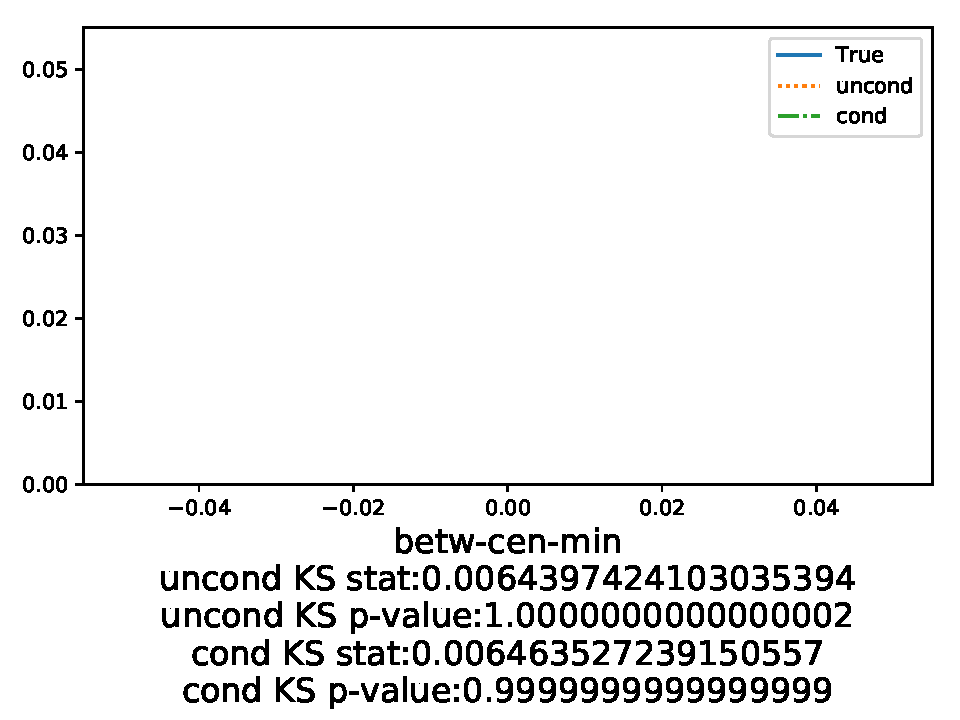
\includegraphics[width=\linewidth]{results/exp1-2/betw-cen-min.pdf} 
		\label{fig:results-noninput-betw-cen-min}
	\end{minipage} 
	
	
	\caption[Graphical results for experiments 1 and 2]{Experiments 1 and 2: Cumulative distribution functions for true data, unconditional network and conditional network for each non-input feature.}
\end{figure}\begin{figure}[ht]
	\begin{minipage}[b]{0.45\linewidth}
		\centering
		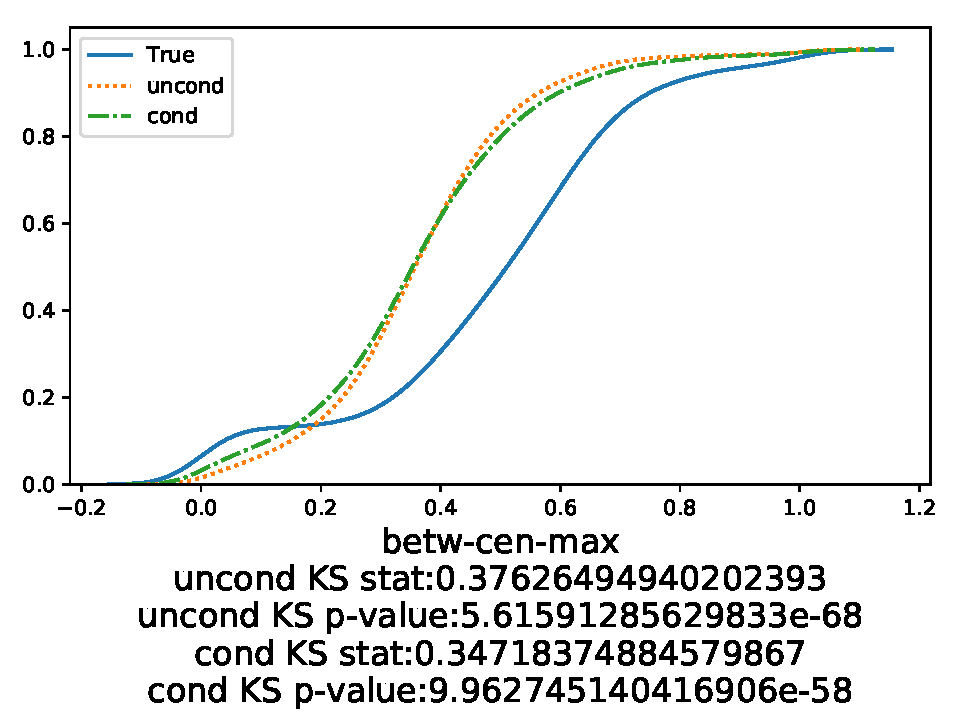
\includegraphics[width=\linewidth]{results/exp1-2/betw-cen-max.pdf} 
		\label{fig:results-noninput-betw-cen-max}
	\end{minipage}
	\begin{minipage}[b]{0.45\linewidth}
		\centering
		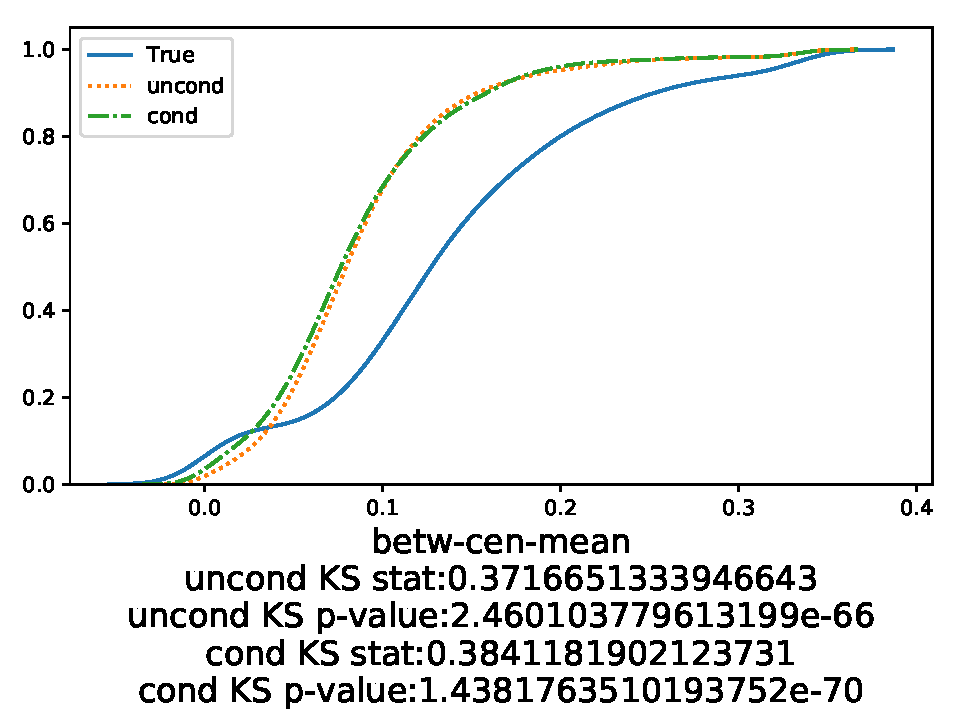
\includegraphics[width=\linewidth]{results/exp1-2/betw-cen-mean.pdf} 
		\label{fig:results-noninput-betw-cen-mean}
	\end{minipage} 
	
	
	\begin{minipage}[b]{0.45\linewidth}
		\centering
		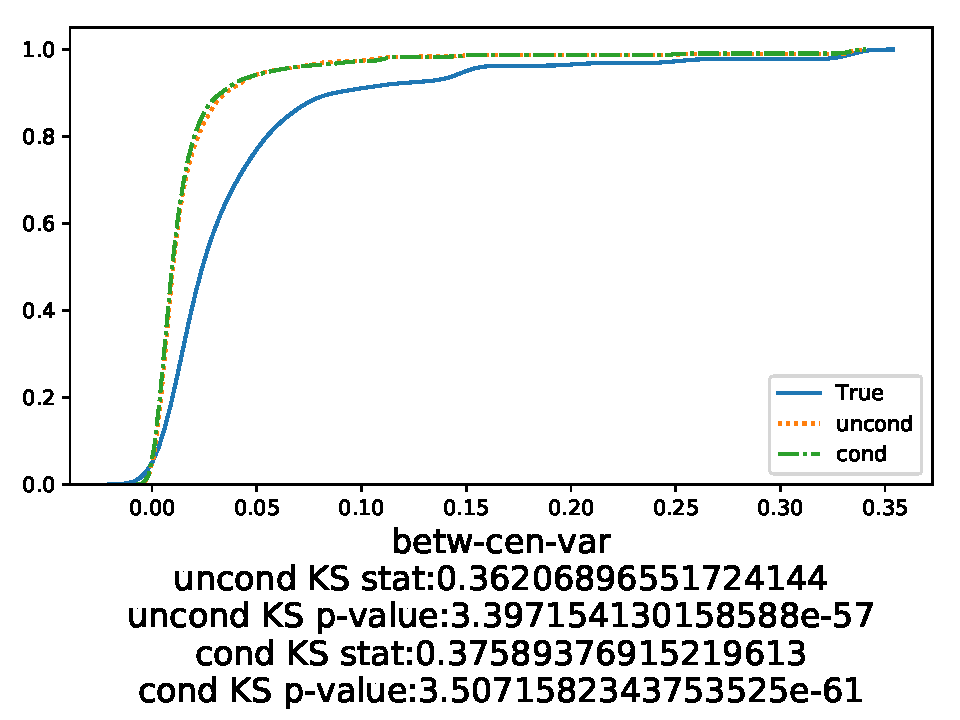
\includegraphics[width=\linewidth]{results/exp1-2/betw-cen-var.pdf} 
		\label{fig:results-noninput-betw-cen-var}
	\end{minipage}
	\begin{minipage}[b]{0.45\linewidth}
		\centering
		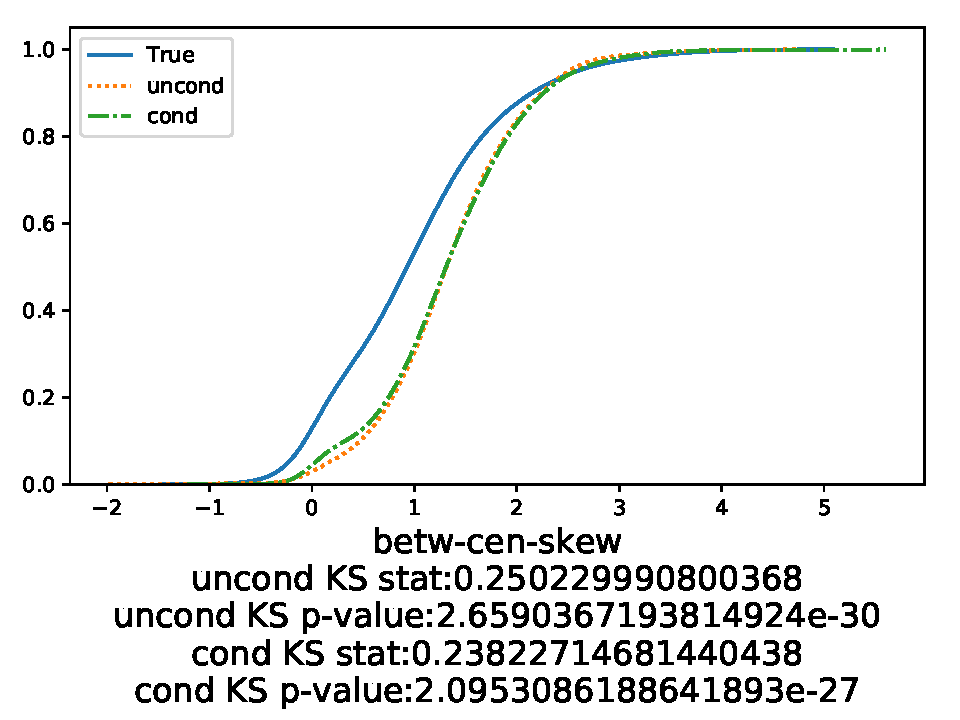
\includegraphics[width=\linewidth]{results/exp1-2/betw-cen-skew.pdf} 
		\label{fig:results-noninput-betw-cen-skew}
	\end{minipage} 
	
	
	\begin{minipage}[b]{0.45\linewidth}
		\centering
		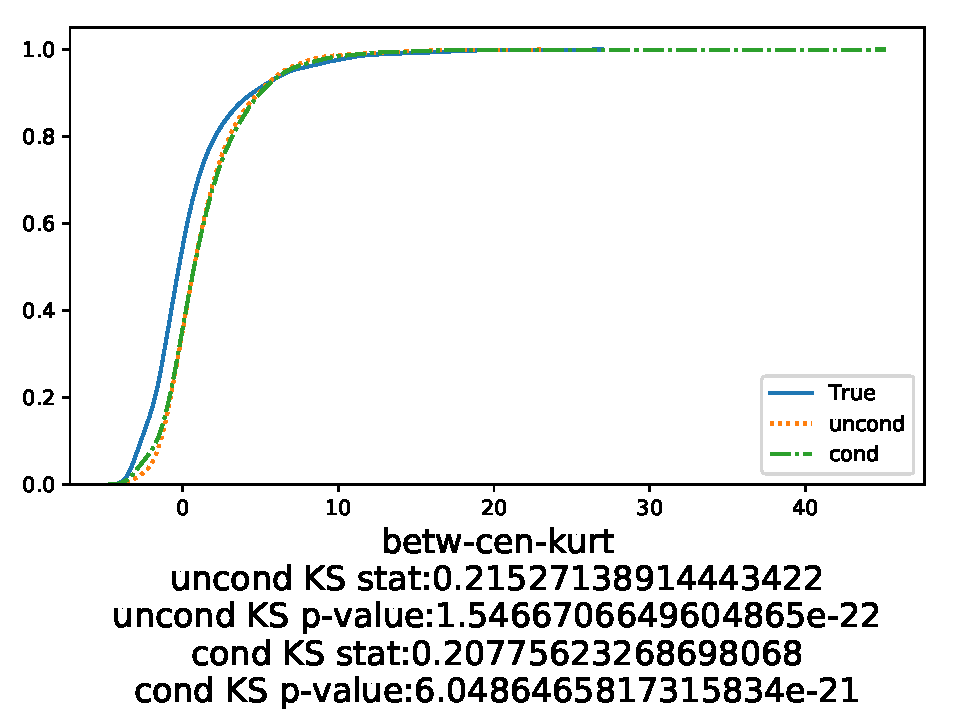
\includegraphics[width=\linewidth]{results/exp1-2/betw-cen-kurt.pdf} 
		\label{fig:results-noninput-betw-cen-kurt}
	\end{minipage}
	\begin{minipage}[b]{0.45\linewidth}
		\centering
		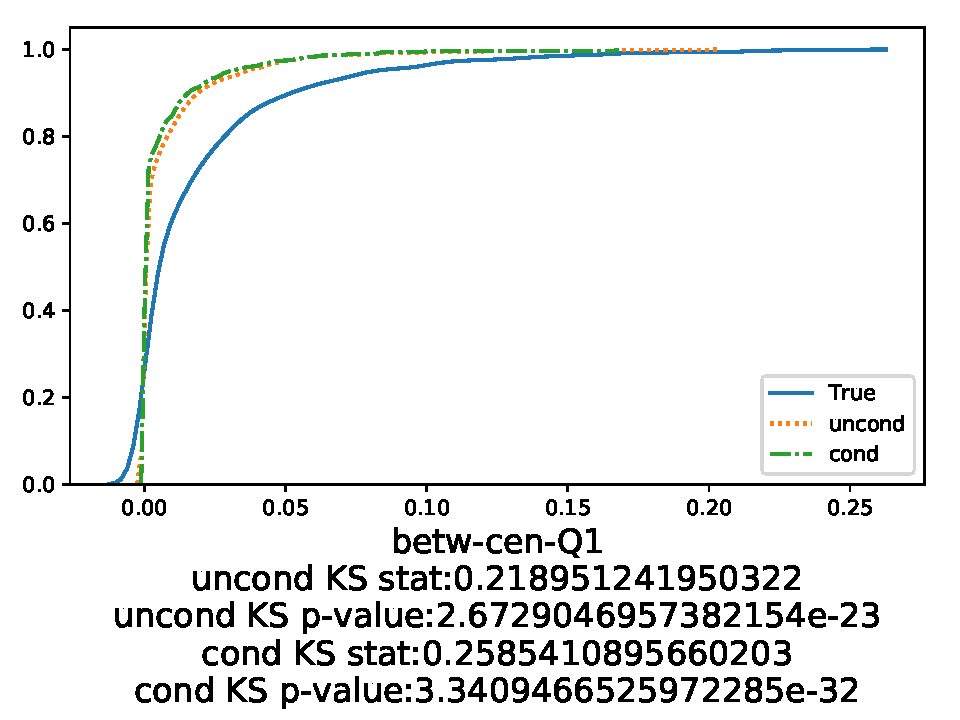
\includegraphics[width=\linewidth]{results/exp1-2/betw-cen-Q1.pdf} 
		\label{fig:results-noninput-betw-cen-Q1}
	\end{minipage} 
	
	
	\caption[Graphical results for experiments 1 and 2]{Experiments 1 and 2: Cumulative distribution functions for true data, unconditional network and conditional network for each non-input feature.}
\end{figure}\begin{figure}[ht]
	\begin{minipage}[b]{0.45\linewidth}
		\centering
		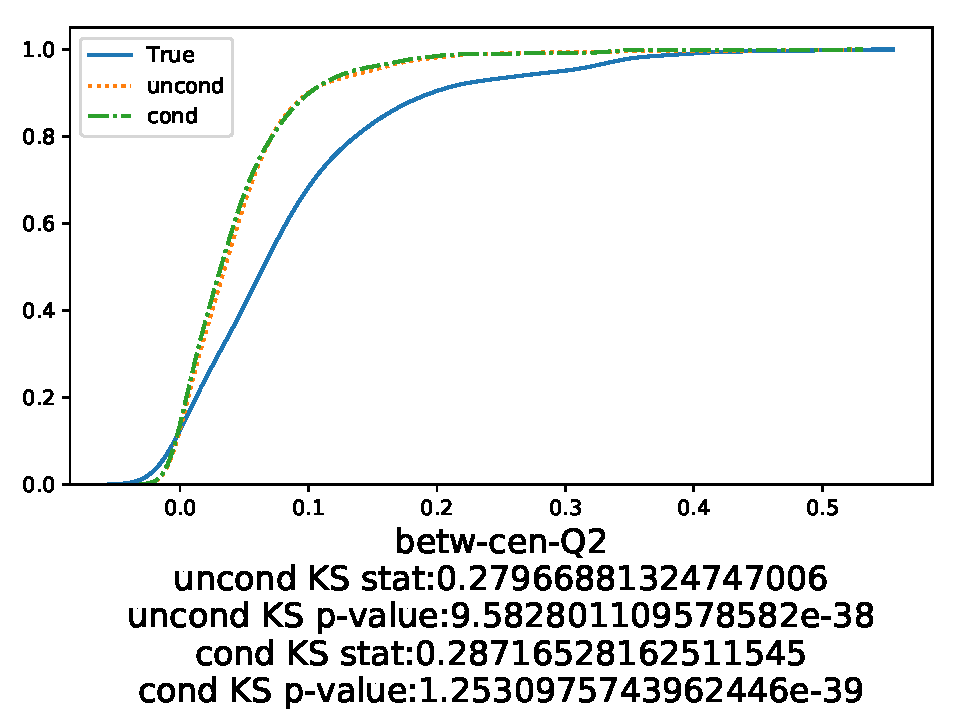
\includegraphics[width=\linewidth]{results/exp1-2/betw-cen-Q2.pdf} 
		\label{fig:results-noninput-betw-cen-Q2}
	\end{minipage}
	\begin{minipage}[b]{0.45\linewidth}
		\centering
		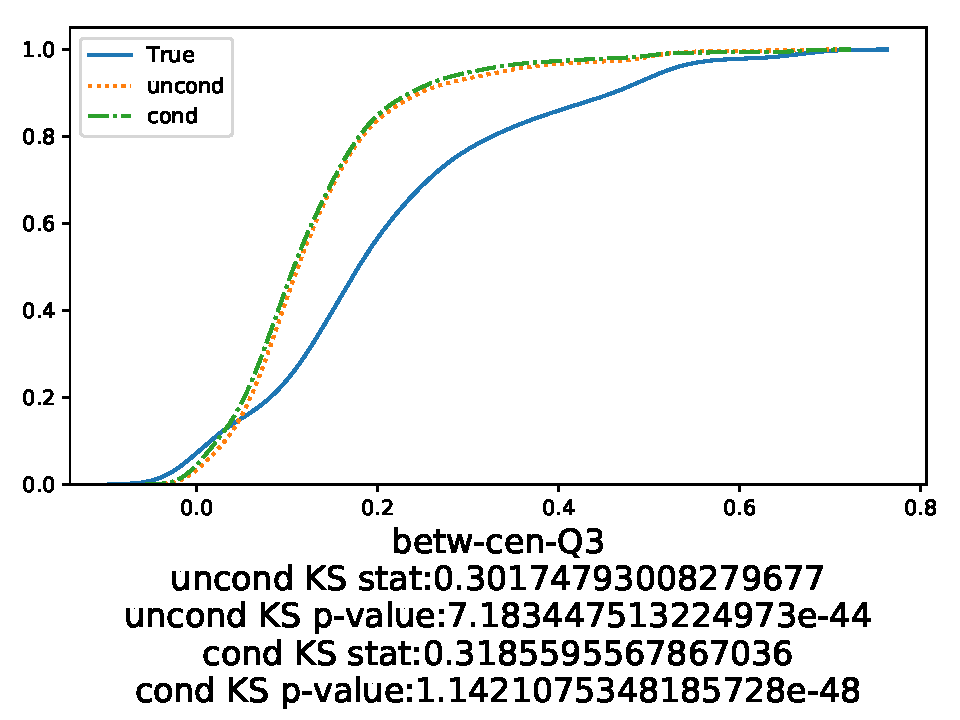
\includegraphics[width=\linewidth]{results/exp1-2/betw-cen-Q3.pdf} 
		\label{fig:results-noninput-betw-cen-Q3}
	\end{minipage} 
	
	
	\begin{minipage}[b]{0.45\linewidth}
		\centering
		\includegraphics[width=\linewidth]{results/exp1-2/closn-cen-min.pdf} 
		\label{fig:results-noninput-closn-cen-min}
	\end{minipage}
	\begin{minipage}[b]{0.45\linewidth}
		\centering
		\includegraphics[width=\linewidth]{results/exp1-2/closn-cen-max.pdf} 
		\label{fig:results-noninput-closn-cen-max}
	\end{minipage} 
	
	
	\begin{minipage}[b]{0.45\linewidth}
		\centering
		\includegraphics[width=\linewidth]{results/exp1-2/closn-cen-mean.pdf} 
		\label{fig:results-noninput-closn-cen-mean}
	\end{minipage}
	\begin{minipage}[b]{0.45\linewidth}
		\centering
		\includegraphics[width=\linewidth]{results/exp1-2/closn-cen-var.pdf} 
		\label{fig:results-noninput-closn-cen-var}
	\end{minipage} 
	
	
	\caption[Graphical results for experiments 1 and 2]{Experiments 1 and 2: Cumulative distribution functions for true data, unconditional network and conditional network for each non-input feature.}
\end{figure}\begin{figure}[ht]
	\begin{minipage}[b]{0.45\linewidth}
		\centering
		\includegraphics[width=\linewidth]{results/exp1-2/closn-cen-skew.pdf} 
		\label{fig:results-noninput-closn-cen-skew}
	\end{minipage}
	\begin{minipage}[b]{0.45\linewidth}
		\centering
		\includegraphics[width=\linewidth]{results/exp1-2/closn-cen-kurt.pdf} 
		\label{fig:results-noninput-closn-cen-kurt}
	\end{minipage} 
	
	
	\begin{minipage}[b]{0.45\linewidth}
		\centering
		\includegraphics[width=\linewidth]{results/exp1-2/closn-cen-Q1.pdf} 
		\label{fig:results-noninput-closn-cen-Q1}
	\end{minipage}
	\begin{minipage}[b]{0.45\linewidth}
		\centering
		\includegraphics[width=\linewidth]{results/exp1-2/closn-cen-Q2.pdf} 
		\label{fig:results-noninput-closn-cen-Q2}
	\end{minipage} 
	
	
	\begin{minipage}[b]{0.45\linewidth}
		\centering
		\includegraphics[width=\linewidth]{results/exp1-2/closn-cen-Q3.pdf} 
		\label{fig:results-noninput-closn-cen-Q3}
	\end{minipage}
	\begin{minipage}[b]{0.45\linewidth}
		\centering
		\includegraphics[width=\linewidth]{results/exp1-2/distmap-max.pdf} 
		\label{fig:results-noninput-distmap-max}
	\end{minipage} 
	
	
	\caption[Graphical results for experiments 1 and 2]{Experiments 1 and 2: Cumulative distribution functions for true data, unconditional network and conditional network for each non-input feature.}
	
\end{figure}\begin{figure}[ht]
	\begin{minipage}[b]{0.45\linewidth}
		\centering
		\includegraphics[width=\linewidth]{results/exp1-2/distmap-mean.pdf} 
		\label{fig:results-noninput-distmap-mean}
	\end{minipage}
	\begin{minipage}[b]{0.45\linewidth}
		\centering
		\includegraphics[width=\linewidth]{results/exp1-2/distmap-var.pdf} 
		\label{fig:results-noninput-distmap-var}
	\end{minipage} 
	
	
	\begin{minipage}[b]{0.45\linewidth}
		\centering
		\includegraphics[width=\linewidth]{results/exp1-2/distmap-Q1.pdf} 
		\label{fig:results-noninput-distmap-Q1}
	\end{minipage}
	\begin{minipage}[b]{0.45\linewidth}
		\centering
		\includegraphics[width=\linewidth]{results/exp1-2/distmap-Q2.pdf} 
		\label{fig:results-noninput-distmap-Q2}
	\end{minipage} 
	
	
	\begin{minipage}[b]{0.45\linewidth}
		\centering
		\includegraphics[width=\linewidth]{results/exp1-2/distmap-Q3.pdf} 
		\label{fig:results-noninput-distmap-Q3}
	\end{minipage}
	
	\caption[Graphical results for experiments 1 and 2]{Experiments 1 and 2: Cumulative distribution functions for true data, unconditional network and conditional network for each non-input feature.}
\end{figure}

